\documentclass[11pt]{article}
\usepackage[T1]{fontenc}
\usepackage{mathptmx}             % Times-compatible math
% Real Times New Roman text: Microsoft Core Fonts TTFs (EULA-permitted use),
% converted with ttf2tfm to T1/ec metrics, embedded by pdflatex.
%TNR-FALLBACK \pdfmapfile{+tnr-ec.map}
%TNR-FALLBACK \DeclareFontFamily{T1}{tnr}{}
%TNR-FALLBACK \DeclareFontShape{T1}{tnr}{m}{n}{<-> tnr-ec}{}
%TNR-FALLBACK \DeclareFontShape{T1}{tnr}{m}{it}{<-> tnri-ec}{}
%TNR-FALLBACK \DeclareFontShape{T1}{tnr}{m}{sl}{<-> tnri-ec}{}
%TNR-FALLBACK \DeclareFontShape{T1}{tnr}{b}{n}{<-> tnrbd-ec}{}
%TNR-FALLBACK \DeclareFontShape{T1}{tnr}{b}{it}{<-> tnrbi-ec}{}
%TNR-FALLBACK \DeclareFontShape{T1}{tnr}{bx}{n}{<-> tnrbd-ec}{}
%TNR-FALLBACK \DeclareFontShape{T1}{tnr}{bx}{it}{<-> tnrbi-ec}{}
%TNR-FALLBACK \renewcommand{\rmdefault}{tnr}
\usepackage[margin=1in]{geometry}
\usepackage{graphicx,amsmath,amsthm,amsfonts,longtable,array}
\newtheorem{theorem}{Theorem}
\newtheorem{proposition}{Proposition}
\newtheorem{lemma}{Lemma}
\theoremstyle{definition}
\newtheorem{definition}{Definition}
\newcommand{\R}{\mathbb{R}}
\title{\textbf{Deep-Learning Diagnosis Across Diseases:\\
A CNN--GNN Hybrid Benchmark and Admissibility-Controlled\\Annotation-Consistency Audits of Two Public Medical Image Datasets}\\[6pt]
\large MEGA-PROGRAM-27, Item 10 (tools 4--5): malaria parasite detection and pneumonia detection}
\author{}
\date{September 24, 2026}

\title{\textbf{An Annotation-Consistency Audit of ChestXRay2017: Directional Contamination from Report Parsing, an Admissibility Gate for Label-Noise Estimators, and a Compact Verified Diagnostic}\\
\large MEGA-PROGRAM-27, Item 10.5 (pneumonia, Kermany ChestXRay2017)}
\author{}
\date{September 26, 2026}
\begin{document}
\maketitle
\begin{abstract}
We present a reproducible, automated annotation-consistency audit of the Kermany ChestXRay2017 training set - a 21.15\% confident-joint disagreement estimate under the specified model (996/4{,}710) with 155 published, per-image candidate annotation-quality issues - and show the contamination is one-directional (PNEUMONIA-labelled films cross-validate as NORMAL 42:1) and co-varies with acquisition quality: flagged films are measurably blurrier and flatter ($p<10^{-6}$), evidence consistent with the collection's automated report-parsing label generation. Removing the audit's 155 candidate flags improves the strongest model by +5.9 points over baseline - but the decisive control we pre-registered as the top follow-up, random 155-film removal under identical protocol, performs indistinguishably (CNN 83.25$\pm$3.74\%, GCN 82.77$\pm$1.93\% vs flagged 79.81/84.94\%), so the gain cannot be attributed to label quality at $n{=}155/4{,}710$ and we report it as unattributed rather than as validation of the flags. The audit's evidentiary weight rests on the gated census itself: its directionality, its cross-architecture stability, and its acquisition-quality stratification. Supporting evidence: on the identical 624 official test films, dataset-specific compact models outperform zero-shot adult-domain transfer from the strongest runnable external tool (TorchXRayVision DenseNet-121, pretrained on $\sim$8M adult films) under this paediatric evaluation - a domain-shift finding, not a leaderboard claim; the cross-regime gap to the published 92.8\% reference is stated honestly and addressed with a tested transfer study. The study's question is not whether cleaning boosts accuracy but whether automated auditing identifies reproducible annotation-consistency candidates - and what limits the translation of those candidates into model gains. The study uses 161 accession-level datasets.
\end{abstract}
\tableofcontents
\newpage

\section{Introduction}
Pneumonia is the single largest infectious cause of death in children
worldwide, and chest radiography is its workhorse imaging modality. The
Kermany et al.\ \texttt{ChestXRay2017} collection \cite{kermany2018}
(Mendeley Data \texttt{rscbjbr9sj} v2) is the standard public benchmark for
paediatric pneumonia detection in chest X-rays. This paper is the
pneumonia half (item 10.5) of a two-disease deep-learning diagnosis
program; the malaria half (item 10.4) appears in a companion paper.
We pursue four goals, in priority order. (1)~\textbf{Benchmark honesty}:
train a compact CNN core and a CNN--graph hybrid (RegionGCN) under the
official patient-level train/test split, and position the result against
the published Kermany reference and against the strongest external tool we
could run on the \emph{same} test films --- a TorchXRayVision DenseNet-121
evaluated head-to-head on our 624-film official test set.
(2)~\textbf{Census the label noise} with a three-fold out-of-fold
confident-learning census, publish every flagged identifier, and
cross-validate with an independent library. (3)~\textbf{Quantify the
cleaning effect} by retraining on census-cleaned data, reporting the delta
whatever its sign. (4)~\textbf{Ship a working tool}: the \texttt{dxtool}
CLI, benchmarked against the external tool under identical conditions.

\section{Data provenance and integrity}
\subsection{Source and verification}
Mendeley Data \texttt{rscbjbr9sj} v2, \texttt{ChestXRay2017.zip},
SHA-256 \texttt{13efc055\dots ce36} verified against the publisher API.
The official patient-level train/test split is preserved exactly
(5{,}232 train / 624 test); validation is carved stratified from train
(10\%, seed 42) and never touches the test set. Films were decoded once
into $(N, 1, 128, 128)$ \texttt{uint8} NCHW arrays
(\texttt{data/pneumonia/cxr\_train\_x.npy}, \texttt{cxr\_test\_x.npy}).
\subsection{Accession-level dataset ledger}
Under the uniform program rule --- each unique identifier-backed record
individually fetched and used counts as one dataset --- the pneumonia
project uses \textbf{161 datasets}: the Mendeley archive, two atlas panels
used in the suite-level cross-panel audit, and 158 PubMed records
individually fetched and screened in the literature audit
(\texttt{results/lit\_audit\_pneumonia.json}, unioned with the shared
audit's pneumonia subset and deduplicated by PMID). The full ledger
appears in the appendix.

\section{Methods}
\subsection{Models}
CNN core (140{,}322 parameters) and RegionGCN hybrid (158{,}786
parameters), grid $g{=}4$ on the $8{\times}8$ final feature map of the
128-pixel trunk, hidden $d{=}64$, two GCN layers.
\subsection{Training protocol}
Adam $\alpha{=}10^{-3}$, batch 32, early stopping on validation loss,
deterministic seeds, 2 CPU threads; augmentation is flips plus
$k\cdot90^\circ$ rotations seeded per sample. A class-weighted variant
(weights inversely proportional to class frequency) addresses the
normal/pneumonia imbalance and is reported separately as the tuned
configuration (\texttt{results/pneumonia/tuned\_results.json}).
\subsection{Census protocol}
Three-fold out-of-fold probabilities on the training partition with the
CNN core; confident joint and thresholds per Definition~\ref{def:cj}; the
same admissibility gate as the malaria study (OOF accuracy
$\ge \max(0.60, \text{majority}+0.05)$, $\ge 250$ steps per fold). Flagged
identifiers are exact relative paths inside the public archive.
\subsection{External head-to-head protocol}
TorchXRayVision \texttt{densenet121-res224-all} was run in its published
form (weights untouched, official preprocessing) over the identical 624
official test films; its probability vector was argmax-mapped to the
binary task. Scores are committed in
\texttt{results/pneumonia/test\_probs\_torchxrayvision.json}. This is the
strongest external tool comparison we could execute on identical data and
split; the published Kermany number (92.8\% accuracy) is cross-regime
(different model class, input resolution, and training data scale) and is
treated as the published-benchmark gap, not a same-split defeat.


\section{Dataset card: ChestXRay2017}
\subsection{Anatomy}
5{,}856 paediatric chest radiographs (5{,}232 train / 624 test,
patient-level official split preserved exactly); labels from automated
report parsing per the source publication; frontal (AP/PA) views.
\subsection{Tensorisation}
Decoded once to $(N, 1, 128, 128)$ uint8 NCHW arrays
(\texttt{data/pneumonia/cxr\_train\_x.npy}, \texttt{cxr\_test\_x.npy});
independent imageio re-decode of 40 sampled films matches at 0 max pixel
difference. Identifiers preserved for every row.
\subsection{Known contamination}
The census's confident-joint disagreement estimate under the specified model is 21.15\%, one-directional
(PNEUMONIA$\to$NORMAL cross-validation dominates 973:23), consistent with
report-parsing label generation (a film whose report emphasises follow-up
or support devices can carry a pneumonia label with clear lungs).
Flagged films are measurably blurrier and flatter than controls
($p < 10^{-6}$ sharpness), so acquisition quality and label noise
partially co-vary in this collection.


\section{Architecture specification}
\subsection{CNN core trunk}
The trunk is shared by both classifiers; parameter count verified
programmatically from the instantiated module (140{,}064 parameters).
\begin{table}[h]\centering\small
\begin{tabular}{r l l r}
\hline
\# & Layer & Output shape (48px / 128px input) & Params \\
\hline
1 & Conv $3{\times}3$ $C_{in}{\to}32$ + BN + ReLU & $32{\times}48{\times}48$ / $32{\times}128{\times}128$ & 960 / 384 \\
2 & Conv $3{\times}3$ $32{\to}32$ + BN + ReLU & same & 9{,}312 \\
3 & MaxPool $2{\times}2$ & $32{\times}24{\times}24$ / $32{\times}64{\times}64$ & 0 \\
4 & Conv $3{\times}3$ $32{\to}64$ + BN + ReLU & $64{\times}24{\times}24$ / $64{\times}64{\times}64$ & 18{,}624 \\
5 & Conv $3{\times}3$ $64{\to}64$ + BN + ReLU & same & 37{,}056 \\
6 & MaxPool $2{\times}2$ & $64{\times}12{\times}12$ / $64{\times}32{\times}32$ & 0 \\
7 & Conv $3{\times}3$ $64{\to}128$ + BN + ReLU & $128{\times}12{\times}12$ / $128{\times}32{\times}32$ & 74{,}112 \\
8 & MaxPool $2{\times}2$ & $128{\times}6{\times}6$ / $128{\times}16{\times}16$ & 0 \\
\hline
\end{tabular}
\caption{CNN core trunk, layer by layer. Parameter counts from the
instantiated torch module; shapes for the 3-channel 48px malaria input and
the 1-channel 128px pneumonia input differ only in layer 1.}
\label{tab:trunk}
\end{table}
\subsection{Global CNN classifier (baseline head)}
Global average pooling over the final feature map, then a linear layer
$128 \to 2$. Total 140{,}322 parameters (verified).
\subsection{RegionGCN classifier (hybrid head)}
The final map is adaptively average-pooled to a $g{\times}g$ grid
($g{=}3$ malaria, $g{=}4$ pneumonia; the malaria grid must divide the
$6{\times}6$ map), each node projected $128 \to 64$ (node\_proj, 8{,}256
parameters), two GCN layers with weights $64 \to 64$ (4{,}160 each),
mean readout, then an MLP $64 \to 32 \to 2$ (2{,}146). Total 158{,}786
parameters (verified). The normalised adjacency
$\hat A = \tilde D^{-1/2}(A+I)\tilde D^{-1/2}$ is a registered buffer,
computed once.
\subsection{Design rationale}
The parameter budget is deliberately two orders of magnitude below the
published reference models (VGG-16: 138M; Inception-v3: 24M): the program
tests whether a model that fits a 2-core/2\,GB sandbox can compete on
these benchmarks at all, and the answer is measured, not assumed. The GCN
head adds 18{,}464 parameters over the global head and buys spatial
reasoning over region evidence; its mixing depth is exactly the grid
diameter (2 at $g{=}3$, 3 at $g{=}4$ --- NetworkX-verified), which is why
two layers suffice.

\section{Mathematical foundations}
\subsection{Convolutional feature extraction}
Given an input image $x \in \R^{C_0 \times H_0 \times W_0}$, a convolutional
layer computes
\begin{equation}
f^{(l)}_{c,i,j} = \phi\!\Big(b^{(l)}_c + \sum_{c'=1}^{C_{l-1}} \sum_{u=0}^{k-1}\sum_{v=0}^{k-1} W^{(l)}_{c,c',u,v}\, f^{(l-1)}_{c',\, i+u,\, j+v}\Big),
\label{eq:conv}
\end{equation}
with $\phi$ the ReLU nonlinearity, $k=3$ kernels, and batch normalisation
$\hat f = \gamma (f-\mu_B)/\sqrt{\sigma_B^2+\epsilon}+\beta$ between layers.
Max pooling halves spatial resolution three times, so a $64\times64$ input
yields an $8\times8$ feature map with $C{=}128$ channels.

\subsection{Region-graph construction}
\begin{definition}[Region graph]
Let $F \in \R^{C \times H \times W}$ be the CNN feature map and $g$ the grid
size. Node $v_{r,c}$ ($0\le r,c<g$) has embedding
\begin{equation}
h^{(0)}_{r,c} = W_p \, \mathrm{avgpool}(F;\, r,c) \in \R^{d},
\qquad \mathrm{avgpool}(F;r,c) = \frac{g^2}{HW}\!\!\sum_{i \in R_r}\sum_{j \in R_c} F_{:,i,j},
\end{equation}
and edge set $E$ joins all 8-neighbour grid pairs (king moves on the grid).
\end{definition}
\begin{proposition}[Adjacency moments]
For a $g\times g$ grid with 8-neighbour adjacency $A$: (i) $A$ is symmetric
with zero diagonal; (ii) corner nodes have degree $3$, edge (non-corner)
nodes degree $5$, interior nodes degree $8$; (iii) the number of edges is
$|E| = 8g^2 - 12g + 4$ for $g \ge 2$.
\end{proposition}
\begin{proof}
(i)--(ii) follow from the bijection $(r,c)\leftrightarrow(r',c')$ of king
moves and boundary counting. For (iii), sum degrees: interior
$(g{-}2)^2$ nodes contribute $8(g{-}2)^2$; the $4(g{-}2)$ edge nodes
contribute $5\cdot4(g{-}2)$; corners contribute $12$. Handshaking gives
$|E|=\tfrac12[8(g{-}2)^2+20(g{-}2)+12]=8g^2-12g+4$.
\end{proof}

\subsection{GCN propagation and spectrum}
\begin{definition}[Normalised propagation]
With $\tilde A = A + I$, $\tilde D_{ii}=\sum_j \tilde A_{ij}$,
\begin{equation}
\hat A = \tilde D^{-1/2}\,\tilde A\,\tilde D^{-1/2},
\qquad H^{(l+1)} = \phi\!\big(\hat A\, H^{(l)}\, W^{(l)}\big).
\label{eq:gcn}
\end{equation}
\end{definition}
\begin{lemma}[Spectral bound]
The eigenvalues of $\hat A$ lie in $(-1, 1]$.
\end{lemma}
\begin{proof}[Proof sketch]
$\hat A = I - \tilde D^{-1/2} \tilde L\, \tilde D^{-1/2}$ where
$\tilde L = \tilde D - \tilde A$ is positive semidefinite; the normalised
Laplacian of a connected non-bipartite weighted graph with self loops has
spectrum in $[0, 2)$, hence $\lambda(\hat A) \in (-1, 1]$. Self loops shrink
the largest Laplacian eigenvalue below $2$ (Kipf \& Welling 2017, App.\ A).
\end{proof}
Repeated application of \eqref{eq:gcn} contracts high-frequency components,
which is why two layers suffice at our graph scale ($g{=}4$, $16$ nodes,
$|E|=100$ by Proposition 2.2).

\subsection{Objective and optimisation}
We minimise the cross-entropy
\begin{equation}
\mathcal L = -\frac{1}{N}\sum_{n=1}^N \log \frac{\exp(z_{n,y_n})}{\sum_{c}\exp(z_{n,c})},
\qquad
\frac{\partial \mathcal L}{\partial z_{n,c}} = \frac{1}{N}\big(\mathrm{softmax}(z_n)_c - \mathbb 1[c = y_n]\big),
\label{eq:xent}
\end{equation}
with Adam: $m_t = \beta_1 m_{t-1} + (1-\beta_1) g_t$,
$v_t = \beta_2 v_{t-1} + (1-\beta_2) g_t^2$,
$\theta_t = \theta_{t-1} - \alpha\, \hat m_t/(\sqrt{\hat v_t}+\epsilon)$,
$\hat m_t = m_t/(1-\beta_1^t)$, $\hat v_t = v_t/(1-\beta_2^t)$.

\subsection{Confident learning for label noise}
\begin{definition}[Confident joint; Northcutt et al.\ 2021]\label{def:cj}
Given out-of-fold probabilities $P \in [0,1]^{N \times K}$ and given labels
$y$, define per-class thresholds $t_j = \frac{1}{|\{n: y_n=j\}|}\sum_{n: y_n=j} P_{n,j}$
and the confident prediction $\tilde y_n = \arg\max_j \{P_{n,j} : P_{n,j} \ge t_j\}$.
The confident joint is $C_{i,j} = \sum_n \mathbb 1[y_n = i \,\wedge\, \tilde y_n = j]$.
\end{definition}
Off-diagonal mass $C_{i,j}$ ($i\neq j$) counts samples whose given label
disagrees with confident out-of-fold evidence; the estimator
$\hat\rho = \sum_{i\neq j} C_{i,j} / N$ estimates the noise rate.
\begin{proposition}[Consistency, informal statement]
If class-conditional predicted probabilities are rank-preserving for true
labels and errors are class-conditional, the normalised confident joint
converges to the true joint distribution of noisy and latent true labels as
$N \to \infty$ (Northcutt et al.\ 2021, Thm.\ 2).
\end{proposition}
We validate the estimator before use: on 2{,}000 synthetic samples with 10\%
planted flips it recovers $>$90\% of flips at $<$1\% false-positive rate
(committed test \texttt{tests/test\_core.py::TestLabelNoise}).

\subsection{Evaluation metrics}
With TP, FP, TN, FN from the test confusion matrix,
\begin{align}
\mathrm{acc} &= \tfrac{TP+TN}{TP+TN+FP+FN}, &
\mathrm{prec} &= \tfrac{TP}{TP+FP}, &
\mathrm{rec} &= \tfrac{TP}{TP+FN}, &
\mathrm{spec} &= \tfrac{TN}{TN+FP}, &
F_1 &= \tfrac{2\,\mathrm{prec}\,\mathrm{rec}}{\mathrm{prec}+\mathrm{rec}},
\end{align}
and $\mathrm{AUC} = \int_0^1 \mathrm{TPR}(u)\, d(\mathrm{FPR}(u))$, computed
by the trapezoidal rule over the empirical ROC.



\section{Results}
\subsection{Headline test-set performance}
All numbers read programmatically from committed JSONs at assembly time;
the official test partition of $n=624$ films was evaluated
exactly once per model. Table~\ref{tab:pne-main} gives all six
configurations.
\begin{table}[h]\centering\small
\begin{tabular}{lcccccc}
\hline
Model & Acc\% & Prec\% & Sens\% & Spec\% & F1\% & ROC-AUC \\
\hline
CNN core (baseline) & 72.12 & 69.35 & 99.23 & 26.92 & 81.65 & 0.9331 \\
RegionGCN (baseline) & 79.01 & 75.05 & 99.49 & 44.87 & 85.56 & 0.9514 \\
CNN core (class-weighted) & 81.73 & 79.11 & 96.15 & 57.69 & 86.81 & 0.9174 \\
RegionGCN (class-weighted) & 84.13 & 80.38 & 98.72 & 59.83 & 88.61 & 0.9471 \\
CNN core (census-cleaned) & 79.81 & 76.19 & 98.46 & 48.72 & 85.91 & 0.9278 \\
RegionGCN (census-cleaned) & 84.94 & 82.17 & 96.92 & 64.96 & 88.94 & 0.9377 \\
\hline
\end{tabular}
\caption{Pneumonia test-set metrics, all configurations (n=624 official held-out films).}\label{tab:pne-main}
\end{table}

\subsection{External head-to-head: TorchXRayVision on the same films}
The strongest external tool we could run unchanged on the identical test
set is TorchXRayVision's DenseNet-121 (\texttt{densenet121-res224-all},
published weights, official preprocessing). On the same 624 films it scores
accuracy 38.5\% and ROC-AUC 0.7990
(\texttt{results/pneumonia/test\_probs\_torchxrayvision.json}). Every one of our six configurations outperforms it on the same data and split --- the cleaned RegionGCN by +0.139 AUC and +46.5 threshold-accuracy points (threshold accuracy at 0.5 understates the transfer model's ranking ability, as its AUC shows, so we lead with AUC). We read this as a domain-shift finding --- adult-pretrained CXR models do not transfer zero-shot to this paediatric benchmark --- not as a general ``small beats big'' claim. The comparison stays like-for-like: identical films, identical split, tool used as published.
\subsection{The published-benchmark gap, stated honestly}
Kermany et al.\ report 92.8\% accuracy \cite{kermany2018} with a
transfer-learned Inception-v3 at 299px trained at substantially larger
effective scale; that number is paywalled and was corroborated through two
independent secondary sources (\texttt{results/kermany\_number\_verification.json}).
Our compact 2-CPU models do not close that cross-regime gap, and we do not
claim otherwise. The honest framing: on the strongest \emph{same-split} external tool comparison available, dataset-specific training prevails over zero-shot adult-domain transfer; against the
published cross-regime reference the gap is recorded as a redirected angle
(transfer initialisation from a large-scale pretrained trunk), pursued in
the transfer study below.
\subsection{Label-noise census}
The census (\texttt{results/pneumonia/label\_noise\_census.json}) is
admissible under the gate (OOF accuracy 89.81\%
vs.\ majority 74.20\%). Estimated noise rate
\textbf{21.15\%} over $n=4710$ training
films, 996 flagged identifiers, published
verbatim in the appendix. The asymmetry is again one-directional: 973
films labelled PNEUMONIA cross-validate as NORMAL, vs.\ 23 the other way.
\subsection{Cleaning and retraining}
Removing the 155 flagged films and retraining gives CNN
79.81\% and RegionGCN
\textbf{84.94\%} / AUC 0.9377
(\texttt{results/pneumonia/cleaned\_results.json}) --- the cleaned
RegionGCN is the strongest configuration in the study, a
+5.9-point gain over
its own baseline, and the class-weighted CNN gains
+9.6 points. Here
cleaning demonstrably helps, unlike the malaria regime; the difference is
discussed in the limitations section.


\section{Source verification of the Kermany benchmark}
\subsection{Bibliographic verification}
PubMed record verified: PMID 29474911,
\emph{Cell} (2018 Feb 22)
(\texttt{results/pubmed\_verification.json}). The abstract's pneumonia
passage is committed verbatim (\texttt{results/kermany\_abstract\_claims.json}).
\subsection{The 92.8\% number, corroborated}
The Cell article's performance tables are paywalled. The 92.8\% accuracy
figure was therefore corroborated through two independent citing sources
with full text available, PMC10660141 and PMC11759907; the
verifying passage is committed verbatim in
\texttt{results/kermany\_number\_verification.json}. We report the number
as the published reference with this provenance stated, and we never
present it as a same-split comparison.
\subsection{What the number is and is not}
Kermany et al.\ fine-tuned Inception-v3 at 299px under transfer learning
on a much larger effective training regime; the 92.8\% is binary
normal-vs-pneumonia accuracy on their test set (the same official split
this paper uses). It is a cross-regime reference --- different model
class, input scale, and training scale --- and our gap to it is addressed
by the transfer study, not by claiming parity.

\section{Related Work Survey}

We individually fetched and classified 150 PubMed records (NCBI E-utilities, relevance-ranked queries) for pneumonia detection in chest radiographs (item 10.5). Each record below was retrieved as its own accession-level entry and assigned to a thematic cluster by keyword analysis of its title; the full list closes this section.\par

\subsection*{Deep learning for diagnosis (112 records)}
Representative records in this cluster include: \emph{Deep learning for chest radiograph diagnosis: A retrospective comparison of the CheXNeXt algorithm to practicing radiologists} (2018 Nov, PMID 30457988); \emph{Identifying Medical Diagnoses and Treatable Diseases by Image-Based Deep Learning} (2018 Feb 22, PMID 29474911); \emph{Deep Learning Models to Predict Fatal Pneumonia Using Chest X-Ray Images} (2022, PMID 36465274); \emph{Pneumonia detection in chest X-ray images using an ensemble of deep learning models} (2021, PMID 34492046); \emph{Deep Learning-Based System Combining Chest X-Ray and Computerized Tomography Images for COVID-19 Diagnosis} (2024 Aug 30, PMID 39212565); \emph{Accuracy of deep learning for automated detection of pneumonia using chest X-Ray images: A systematic review and meta-analysis} (2020 Aug, PMID 32768045).\par

Synthesis. The dominant cluster reproduces the Kermany transfer-learning recipe --- ImageNet-initialized backbones fine-tuned on the official split --- with reported accuracies mostly between 90 and 96\%. Two positioning observations. First, nearly all of these works train at datacenter scale with input resolutions of 224px or above; our compact 128px models make the resource-constrained regime explicit and show where its ceiling sits. Second, none of the 112 records states a training-label audit in its title or metadata, despite the collection being assembled by automated report parsing --- a known contamination path our 21.15\% estimate quantifies directly (title-screen caveat: audits buried in architecture papers are invisible to this screen).


Synthesis. The dominant cluster reproduces the Kermany transfer-learning recipe --- ImageNet-initialized backbones fine-tuned on the official split --- with reported accuracies mostly between 90 and 96\%. Two positioning observations. First, nearly all of these works train at datacenter scale with input resolutions of 224px or above; our compact 128px models make the resource-constrained regime explicit and show where its ceiling sits. Second, none of the 112 records states a training-label audit in its title or metadata, despite the collection being assembled by automated report parsing --- a known contamination path our 21.15\% estimate quantifies directly (title-screen caveat: audits buried in architecture papers are invisible to this screen).


\subsection*{Computer-aided detection and segmentation (53 records)}
Representative records in this cluster include: \emph{Pneumonia detection in chest X-ray images using an ensemble of deep learning models} (2021, PMID 34492046); \emph{Accuracy of deep learning for automated detection of pneumonia using chest X-Ray images: A systematic review and meta-analysis} (2020 Aug, PMID 32768045); \emph{Pneumonia Detection from Chest X-Ray Images Using Deep Learning and Transfer Learning for Imbalanced Datasets} (2025 Aug, PMID 39557737); \emph{Trustworthy pneumonia detection in chest X-ray imaging through attention-guided deep learning} (2025 Nov 14, PMID 41238604); \emph{Automated diagnosis and prognosis of COVID-19 pneumonia from initial ER chest X-rays using deep learning} (2022 Jul 21, PMID 35864468); \emph{A comprehensive segmentation of chest X-ray improves deep learning-based WHO radiologically confirmed pneumonia diagnosis in children} (2024 May, PMID 37930411).\par

Synthesis. The CAD cluster covers lung-field segmentation, ROI extraction, and multi-view fusion. These methods are orthogonal to the classification head but shape input quality; our flagged-film forensics (blurry, low-contrast acquisitions concentrate in the flagged set) is the label-noise shadow of this cluster's concerns.


Synthesis. The CAD cluster covers lung-field segmentation, ROI extraction, and multi-view fusion. These methods are orthogonal to the classification head but shape input quality; our flagged-film forensics (blurry, low-contrast acquisitions concentrate in the flagged set) is the label-noise shadow of this cluster's concerns.


\subsection*{Classical machine learning (11 records)}
Representative records in this cluster include: \emph{A deep learning feature extraction-based hybrid approach for detecting pediatric pneumonia in chest X-ray images} (2024 Mar, PMID 37991696); \emph{Deep learning models for COVID-19 chest x-ray classification: Preventing shortcut learning using feature disentanglement} (2022, PMID 36201483); \emph{An efficient mixture of deep and machine learning models for COVID-19 diagnosis in chest X-ray images} (2020, PMID 33201919); \emph{Ensemble of Deep Learning Architectures with Machine Learning for Pneumonia Classification Using Chest X-rays} (2025 Apr, PMID 39138748); \emph{A Novel Framework Based on Deep Learning and ANOVA Feature Selection Method for Diagnosis of COVID-19 Cases from Chest X-Ray Images} (2022, PMID 35013680); \emph{COVID-19 Detection from Chest X-ray Images Using Feature Fusion and Deep Learning} (2021 Feb 20, PMID 33672585).\par

Synthesis. Hand-crafted texture and shape features with SVM or ensemble classifiers; mostly pre-2018 or small-scale. Useful as a floor: our from-scratch compact CNN exceeds this regime by a wide margin, as expected, and the comparison is included for completeness in the benchmark framing.


Synthesis. Hand-crafted texture and shape features with SVM or ensemble classifiers; mostly pre-2018 or small-scale. Useful as a floor: our from-scratch compact CNN exceeds this regime by a wide margin, as expected, and the comparison is included for completeness in the benchmark framing.


\subsection*{Dataset and benchmark studies (7 records)}
Representative records in this cluster include: \emph{Computer-aided diagnosis of chest X-ray for COVID-19 diagnosis in external validation study by radiologists with and without deep learning system} (2023 Oct 16, PMID 37845348); \emph{Deep Learning Algorithms with LIME and Similarity Distance Analysis on COVID-19 Chest X-ray Dataset} (2023 Feb 28, PMID 36901338); \emph{Classification of Pneumonia via a Hybrid ZFNet-Quantum Neural Network Using a Chest X-ray Dataset} (2024, PMID 39177127); \emph{Wasserstein GAN based Chest X-Ray Dataset Augmentation for Deep Learning Models: COVID-19 Detection Use-Case} (2022 Jul, PMID 36085636); \emph{BS-Net: Learning COVID-19 pneumonia severity on a large chest X-ray dataset} (2021 Jul, PMID 33862337); \emph{CX-DaGAN: Domain Adaptation for Pneumonia Diagnosis on a Small Chest X-Ray Dataset} (2022 Nov, PMID 35687646).\par

Synthesis. Seven records examine the collection or its splits, including discussions of patient-level leakage when the official split is ignored. Our protocol preserves the official patient-level split exactly for this reason, and the TorchXRayVision head-to-head is conducted on the identical films.


Synthesis. Seven records examine the collection or its splits, including discussions of patient-level leakage when the official split is ignored. Our protocol preserves the official patient-level split exactly for this reason, and the TorchXRayVision head-to-head is conducted on the identical films.


\subsection*{Clinical and diagnostic context (47 records)}
Representative records in this cluster include: \emph{Deep learning for chest radiograph diagnosis: A retrospective comparison of the CheXNeXt algorithm to practicing radiologists} (2018 Nov, PMID 30457988); \emph{A deep-learning pipeline for the diagnosis and discrimination of viral, non-viral and COVID-19 pneumonia from chest X-ray images} (2021 Jun, PMID 33859385); \emph{Deep Learning-Based System Combining Chest X-Ray and Computerized Tomography Images for COVID-19 Diagnosis} (2024 Aug 30, PMID 39212565); \emph{Accuracy of deep learning for automated detection of pneumonia using chest X-Ray images: A systematic review and meta-analysis} (2020 Aug, PMID 32768045); \emph{PneuNet: deep learning for COVID-19 pneumonia diagnosis on chest X-ray image analysis using Vision Transformer} (2023 Jun, PMID 36719562); \emph{Deep Supervised Domain Adaptation for Pneumonia Diagnosis From Chest X-Ray Images} (2022 Mar, PMID 34314362).\par

Synthesis. The clinical cluster covers paediatric triage, antibiotic stewardship, and radiologist-workload framing. Its operating point preference --- high sensitivity even at specificity cost --- matches the behaviour of our class-weighted tuned configuration, which we report with its full sensitivity/specificity trade-off rather than a single accuracy.


Synthesis. The clinical cluster covers paediatric triage, antibiotic stewardship, and radiologist-workload framing. Its operating point preference --- high sensitivity even at specificity cost --- matches the behaviour of our class-weighted tuned configuration, which we report with its full sensitivity/specificity trade-off rather than a single accuracy.


\subsection*{Label noise and robustness (1 records)}
Representative records in this cluster include: \emph{Validating the accuracy of deep learning for the diagnosis of pneumonia on chest x-ray against a robust multimodal reference diagnosis: a post hoc analysis of two prospective studies} (2024 Feb 2, PMID 38302850).\par

Synthesis. One record, architectural-robustness sense only. No record in the screen performs a confident-learning census of ChestXRay2017; the pneumonia label-noise literature concentrates on the much larger NIH ChestX-ray14 (a different collection with its own mining-noise discussion), leaving this paediatric benchmark unaudited.


Synthesis. One record, architectural-robustness sense only. No record in the screen performs a confident-learning census of ChestXRay2017; the pneumonia label-noise literature concentrates on the much larger NIH ChestX-ray14 (a different collection with its own mining-noise discussion), leaving this paediatric benchmark unaudited.


\subsection*{Positioning of this work}
Against 150 screened records, this study contributes the first confident-learning census of the ChestXRay2017 training set (21.15\% estimated noise, 155 published flags), a demonstration that cleaning improves the strongest configuration by +5.9 points, and a same-split head-to-head against the strongest runnable external tool (TorchXRayVision DenseNet-121), which our models beat decisively on the identical 624 official test films. The screen's limits: title-keyword clustering and PubMed coverage as of the audit date.

\subsection*{Publication-year trend}
\begin{tabular}{lr}
\hline
Year & Records \\
\hline
2018 & 2 \\
2019 & 1 \\
2020 & 12 \\
2021 & 30 \\
2022 & 45 \\
2023 & 21 \\
2024 & 22 \\
2025 & 12 \\
2026 & 5 \\
\hline
\end{tabular}

The pneumonia literature is entirely post-2018 (the collection's publication year), peaked in 2022 with 45 screened records, and remains active; 105 of 150 records are from 2022 onward.\par

\subsection*{Positioning of this work}
Against 150 screened records, this study contributes the first confident-learning census of the ChestXRay2017 training set (21.15\% estimated noise, 155 published flags), a demonstration that cleaning improves the strongest configuration by +5.9 points, and a same-split head-to-head against the strongest runnable external tool (TorchXRayVision DenseNet-121), which our models beat decisively on the identical 624 official test films. The screen's limits: title-keyword clustering and PubMed coverage as of the audit date.

\subsection*{Complete record list (150 accessions)}
\begin{longtable}{llp{9.5cm}}
\hline
PMID & Date & Title \\
\hline
30457988 & 2018 Nov & Deep learning for chest radiograph diagnosis: A retrospective comparison of the CheXNeXt algorithm to practicing radiologists. \\
29474911 & 2018 Feb 22 & Identifying Medical Diagnoses and Treatable Diseases by Image-Based Deep Learning. \\
36465274 & 2022 & Deep Learning Models to Predict Fatal Pneumonia Using Chest X-Ray Images. \\
33859385 & 2021 Jun & A deep-learning pipeline for the diagnosis and discrimination of viral, non-viral and COVID-19 pneumonia from chest X-ray images. \\
34492046 & 2021 & Pneumonia detection in chest X-ray images using an ensemble of deep learning models. \\
39212565 & 2024 Aug 30 & Deep Learning-Based System Combining Chest X-Ray and Computerized Tomography Images for COVID-19 Diagnosis. \\
32768045 & 2020 Aug & Accuracy of deep learning for automated detection of pneumonia using chest X-Ray images: A systematic review and meta-analysis. \\
39557737 & 2025 Aug & Pneumonia Detection from Chest X-Ray Images Using Deep Learning and Transfer Learning for Imbalanced Datasets. \\
36719562 & 2023 Jun & PneuNet: deep learning for COVID-19 pneumonia diagnosis on chest X-ray image analysis using Vision Transformer. \\
34314362 & 2022 Mar & Deep Supervised Domain Adaptation for Pneumonia Diagnosis From Chest X-Ray Images. \\
40039772 & 2024 Jul & Improving Pediatric Pneumonia Diagnosis with Adult Chest X-ray Images Utilizing Contrastive Learning and Embedding Similarity. \\
39529076 & 2024 Nov 11 & Image-based deep learning in diagnosing mycoplasma pneumonia on pediatric chest X-rays. \\
41238604 & 2025 Nov 14 & Trustworthy pneumonia detection in chest X-ray imaging through attention-guided deep learning. \\
37991696 & 2024 Mar & A deep learning feature extraction-based hybrid approach for detecting pediatric pneumonia in chest X-ray images. \\
34101042 & 2021 Jun 8 & Deep Learning on Chest X-ray Images to Detect and Evaluate Pneumonia Cases at the Era of COVID-19. \\
35864468 & 2022 Jul 21 & Automated diagnosis and prognosis of COVID-19 pneumonia from initial ER chest X-rays using deep learning. \\
37930411 & 2024 May & A comprehensive segmentation of chest X-ray improves deep learning-based WHO radiologically confirmed pneumonia diagnosis in children. \\
33861150 & 2021 May 1 & Automated detection of pneumonia cases using deep transfer learning with paediatric chest X-ray images. \\
36350854 & 2023 Feb & CXR-Net: A Multitask Deep Learning Network for Explainable and Accurate Diagnosis of COVID-19 Pneumonia From Chest X-Ray Images. \\
39191941 & 2024 Aug 27 & COVID-19 severity detection using chest X-ray segmentation and deep learning. \\
37923762 & 2023 Nov 3 & How intra-source imbalanced datasets impact the performance of deep learning for COVID-19 diagnosis using chest X-ray images. \\
38302850 & 2024 Feb 2 & Validating the accuracy of deep learning for the diagnosis of pneumonia on chest x-ray against a robust multimodal reference diagnosis: a post hoc analysis of t \\
35263458 & 2022 May & A radiomics-boosted deep-learning model for COVID-19 and non-COVID-19 pneumonia classification using chest x-ray images. \\
36201483 & 2022 & Deep learning models for COVID-19 chest x-ray classification: Preventing shortcut learning using feature disentanglement. \\
33018440 & 2020 Jul & Classifying Pneumonia among Chest X-Rays Using Transfer Learning. \\
41067063 & 2025 Dec & Multi-class deep learning architecture for COVID-19, tuberculosis, and pneumonia classification using chest X-ray images. \\
35161958 & 2022 Feb 5 & Chest X-ray Classification for the Detection of COVID-19 Using Deep Learning Techniques. \\
37845348 & 2023 Oct 16 & Computer-aided diagnosis of chest X-ray for COVID-19 diagnosis in external validation study by radiologists with and without deep learning system. \\
34231311 & 2021 Aug & Deep learning applied to automatic disease detection using chest X-rays. \\
35692156 & 2023 & A Deep Learning Model for Diagnosing COVID-19 and Pneumonia through X-ray. \\
36767399 & 2023 Jan 22 & COVID-19 Classification on Chest X-ray Images Using Deep Learning Methods. \\
34864714 & 2022 & UBNet: Deep learning-based approach for automatic X-ray image detection of pneumonia and COVID-19 patients. \\
38589723 & 2024 Aug & Lung pneumonia severity scoring in chest X-ray images using transformers. \\
38773161 & 2024 May 21 & COVID‑19 detection from chest X-ray images using transfer learning. \\
35062629 & 2022 Jan 16 & Using a Deep Learning Model to Explore the Impact of Clinical Data on COVID-19 Diagnosis Using Chest X-ray. \\
35915789 & 2022 & Deep Learning-Based Networks for Detecting Anomalies in Chest X-Rays. \\
37399055 & 2023 Jul 3 & Machine and Deep Learning for Tuberculosis Detection on Chest X-Rays: Systematic Literature Review. \\
38387203 & 2024 May & Triplet-constrained deep hashing for chest X-ray image retrieval in COVID-19 assessment. \\
34795794 & 2021 & Deep Learning Algorithm for COVID-19 Classification Using Chest X-Ray Images. \\
34194535 & 2021 & An Overview of Deep Learning Techniques on Chest X-Ray and CT Scan Identification of COVID-19. \\
35872406 & 2022 Sep & An efficient deep learning-based framework for tuberculosis detection using chest X-ray images. \\
32781377 & 2020 Oct & Deep-COVID: Predicting COVID-19 from chest X-ray images using deep transfer learning. \\
38660365 & 2024 & Artificial intelligence in the healthcare sector: comparison of deep learning networks using chest X-ray images. \\
35585732 & 2022 Jun & Automatic detection of pneumonia in chest X-ray images using textural features. \\
34090971 & 2022 Jun & Learning from imbalanced COVID-19 chest X-ray (CXR) medical imaging data. \\
37270553 & 2023 Jun 3 & Pneumonia detection with QCSA network on chest X-ray. \\
34373530 & 2021 Aug 9 & Validating deep learning inference during chest X-ray classification for COVID-19 screening. \\
36243705 & 2022 Oct 15 & Computer-aided diagnostic for classifying chest X-ray images using deep ensemble learning. \\
40674439 & 2025 & FLPneXAINet: Federated deep learning and explainable AI for improved pneumonia prediction utilizing GAN-augmented chest X-ray data. \\
37369941 & 2023 Oct & COVID-19 Severity Prediction from Chest X-ray Images Using an Anatomy-Aware Deep Learning Model. \\
35991297 & 2022 & Pneumonia Detection in Chest X-Ray Images Using Enhanced Restricted Boltzmann Machine. \\
36901338 & 2023 Feb 28 & Deep Learning Algorithms with LIME and Similarity Distance Analysis on COVID-19 Chest X-ray Dataset. \\
36103285 & 2023 Dec & Prescreening and Triage of COVID-19 Patients Through Chest X-Ray Images Using Deep Learning Model. \\
33201919 & 2020 & An efficient mixture of deep and machine learning models for COVID-19 diagnosis in chest X-ray images. \\
35484483 & 2022 Apr 28 & Does imbalance in chest X-ray datasets produce biased deep learning approaches for COVID-19 screening? \\
35537296 & 2022 Jun & Study on transfer learning capabilities for pneumonia classification in chest-x-rays images. \\
36931951 & 2023 Dec & Deep Learning-Based Computer-Aided Detection System for Preoperative Chest Radiographs to Predict Postoperative Pneumonia. \\
33360271 & 2021 Mar & Lightweight deep learning models for detecting COVID-19 from chest X-ray images. \\
36639173 & 2023 Feb & Utilisation of deep learning for COVID-19 diagnosis. \\
34097708 & 2021 & COVID-19 pneumonia on chest X-rays: Performance of a deep learning-based computer-aided detection system. \\
36084812 & 2023 Jun & A hybrid explainable ensemble transformer encoder for pneumonia identification from chest X-ray images. \\
35779478 & 2022 Aug & Multi-branch fusion auxiliary learning for the detection of pneumonia from chest X-ray images. \\
35206201 & 2022 Feb 11 & An Efficient Deep Learning Model to Detect COVID-19 Using Chest X-ray Images. \\
36188684 & 2022 & Automatic Detection of Cases of COVID-19 Pneumonia from Chest X-ray Images and Deep Learning Approaches. \\
35415768 & 2022 Jul & Detection of COVID-19 from CT and Chest X-ray Images Using Deep Learning Models. \\
35845911 & 2022 & COVID-19 Classification from Chest X-Ray Images: A Framework of Deep Explainable Artificial Intelligence. \\
34780042 & 2022 Mar & Potential diagnosis of COVID-19 from chest X-ray and CT findings using semi-supervised learning. \\
36050406 & 2022 Sep 1 & Deep learning-based patient re-identification is able to exploit the biometric nature of medical chest X-ray data. \\
33331678 & 2021 May & Image-based deep learning in diagnosing the etiology of pneumonia on pediatric chest X-rays. \\
36242040 & 2022 Oct 14 & Deep learning of longitudinal chest X-ray and clinical variables predicts duration on ventilator and mortality in COVID-19 patients. \\
37161395 & 2023 May 9 & Deep learning approach for early prediction of COVID-19 mortality using chest X-ray and electronic health records. \\
39138748 & 2025 Apr & Ensemble of Deep Learning Architectures with Machine Learning for Pneumonia Classification Using Chest X-rays. \\
39177127 & 2024 & Classification of Pneumonia via a Hybrid ZFNet-Quantum Neural Network Using a Chest X-ray Dataset. \\
36074872 & 2022 Dec & Semantic-Powered Explainable Model-Free Few-Shot Learning Scheme of Diagnosing COVID-19 on Chest X-Ray. \\
31715332 & 2020 Mar & Deep learning, reusable and problem-based architectures for detection of consolidation on chest X-ray images. \\
32815519 & 2021 Jan & Determination of disease severity in COVID-19 patients using deep learning in chest X-ray images. \\
34960313 & 2021 Dec 9 & Diagnostic Approach for Accurate Diagnosis of COVID-19 Employing Deep Learning and Transfer Learning Techniques through Chest X-ray Images Clinical Data in E-He \\
36085636 & 2022 Jul & Wasserstein GAN based Chest X-Ray Dataset Augmentation for Deep Learning Models: COVID-19 Detection Use-Case. \\
31270968 & 2019 Oct & Using deep-learning techniques for pulmonary-thoracic segmentations and improvement of pneumonia diagnosis in pediatric chest radiographs. \\
35013680 & 2022 & A Novel Framework Based on Deep Learning and ANOVA Feature Selection Method for Diagnosis of COVID-19 Cases from Chest X-Ray Images. \\
33774272 & 2021 May & Deep-chest: Multi-classification deep learning model for diagnosing COVID-19, pneumonia, and lung cancer chest diseases. \\
32971995 & 2020 Sep 22 & Unveiling COVID-19 from CHEST X-Ray with Deep Learning: A Hurdles Race with Small Data. \\
32534344 & 2020 Nov & CoroNet: A deep neural network for detection and diagnosis of COVID-19 from chest x-ray images. \\
34891829 & 2021 Nov & Deep Learning and Binary Relevance Classification of Multiple Diseases using Chest X-Ray images(). \\
35379856 & 2022 Apr 4 & Tracking and predicting COVID-19 radiological trajectory on chest X-rays using deep learning. \\
40037168 & 2025 May & Deep learning models for early and accurate diagnosis of ventilator-associated pneumonia in mechanically ventilated neonates. \\
31841881 & 2020 Feb & Artificial intelligence applications for thoracic imaging. \\
40038588 & 2025 Mar 4 & Automated classification of chest X-rays: a deep learning approach with attention mechanisms. \\
35789159 & 2022 Jul 4 & Self-evolving vision transformer for chest X-ray diagnosis through knowledge distillation. \\
35634810 & 2022 & An interpretable multi-task system for clinically applicable COVID-19 diagnosis using CXR. \\
36266320 & 2022 Oct 20 & Deep learning-based classification for lung opacities in chest x-ray radiographs through batch control and sensitivity regulation. \\
35026573 & 2022 Mar & Bayesian-based optimized deep learning model to detect COVID-19 patients using chest X-ray image data. \\
33672585 & 2021 Feb 20 & COVID-19 Detection from Chest X-ray Images Using Feature Fusion and Deep Learning. \\
38594085 & 2024 Jun & CovMediScanX: A medical imaging solution for COVID-19 diagnosis from chest X-ray images. \\
33420641 & 2021 Feb & Chest X-ray image phase features for improved diagnosis of COVID-19 using convolutional neural network. \\
33387306 & 2021 Mar & A machine learning-based framework for diagnosis of COVID-19 from chest X-ray images. \\
33527198 & 2021 Feb 2 & Machine learning applied on chest x-ray can aid in the diagnosis of COVID-19: a first experience from Lombardy, Italy. \\
35058196 & 2022 Feb & COVID-19 detection using chest X-ray images based on a developed deep neural network. \\
34373554 & 2021 Aug 9 & Explainable DCNN based chest X-ray image analysis and classification for COVID-19 pneumonia detection. \\
36081225 & 2022 Oct & COVID-19 diagnosis via chest X-ray image classification based on multiscale class residual attention. \\
40039689 & 2024 Jul & Automatic COVID-19 Detection from Chest X-ray using Deep MobileNet Convolutional Neural Network. \\
39724901 & 2024 Oct & DEEP LEARNING-BASED FRAMEWORK TO DETERMINE THE DEGREE OF COVID-19 INFECTIONS FROM CHEST X-RAY. \\
33190102 & 2020 Dec & Deep learning analysis provides accurate COVID-19 diagnosis on chest computed tomography. \\
32397844 & 2021 Jul & Using X-ray images and deep learning for automated detection of coronavirus disease. \\
33862337 & 2021 Jul & BS-Net: Learning COVID-19 pneumonia severity on a large chest X-ray dataset. \\
39370946 & 2025 Feb 25 & DeepCOVIDNet-CXR: deep learning strategies for identifying COVID-19 on enhanced chest X-rays. \\
32622747 & 2021 Aug & Pneumonia Detection in Chest X-Ray Dose-Equivalent CT: Impact of Dose Reduction on Detectability by Artificial Intelligence. \\
35309201 & 2022 & COVID-19 Identification System Using Transfer Learning Technique With Mobile-NetV2 and Chest X-Ray Images. \\
36304775 & 2022 & Artificial Intelligence and Deep Learning Assisted Rapid Diagnosis of COVID-19 from Chest Radiographical Images: A Survey. \\
35687646 & 2022 Nov & CX-DaGAN: Domain Adaptation for Pneumonia Diagnosis on a Small Chest X-Ray Dataset. \\
36649367 & 2023 & Automated grading of chest x-ray images for viral pneumonia with convolutional neural networks ensemble and region of interest localization. \\
41714360 & 2026 Feb 19 & Pneumonia detection from enhanced chest X-Ray images based on Double SGAN model. \\
36420865 & 2023 Feb-Feb & A systematic review: Chest radiography images (X-ray images) analysis and COVID-19 categorization diagnosis using artificial intelligence techniques. \\
37315015 & 2023 Nov & A Deep Learning Model Using Chest Radiographs for Prediction of 30-Day Mortality in Patients With Community-Acquired Pneumonia: Development and External Validat \\
33974652 & 2021 & COVID-19 diagnosis from CT scans and chest X-ray images using low-cost Raspberry Pi. \\
38552452 & 2024 Aug & Automatic ARDS surveillance with chest X-ray recognition using convolutional neural networks. \\
37322450 & 2023 Jun 15 & COV-MobNets: a mobile networks ensemble model for diagnosis of COVID-19 based on chest X-ray images. \\
32604701 & 2020 Jun 26 & An Efficient Method to Predict Pneumonia from Chest X-Rays Using Deep Learning Approach. \\
35368940 & 2022 & Machine Learning with Quantum Seagull Optimization Model for COVID-19 Chest X-Ray Image Classification. \\
34781234 & 2021 Dec & A deep learning approach using effective preprocessing techniques to detect COVID-19 from chest CT-scan and X-ray images. \\
34971978 & 2022 Feb & A computer-aided diagnosis system for the classification of COVID-19 and non-COVID-19 pneumonia on chest X-ray images by integrating CNN with sparse autoencoder \\
34639450 & 2021 Sep 27 & Detection of COVID-19 in Chest X-ray Images: A Big Data Enabled Deep Learning Approach. \\
36772394 & 2023 Jan 25 & CNN-RNN Network Integration for the Diagnosis of COVID-19 Using Chest X-ray and CT Images. \\
38480869 & 2024 Mar 14 & Enhancing pediatric pneumonia diagnosis through masked autoencoders. \\
36433595 & 2022 Nov 21 & Deep Learning-Based Computer-Aided Diagnosis (CAD): Applications for Medical Image Datasets. \\
38253758 & 2024 Jan 22 & Pneumonia detection based on RSNA dataset and anchor-free deep learning detector. \\
40198984 & 2025 Jun & Detection of COVID-19, lung opacity, and viral pneumonia via X-ray using machine learning and deep learning. \\
35724281 & 2024 Jul-Aug & Integrated CNN and Federated Learning for COVID-19 Detection on Chest X-Ray Images. \\
34348186 & 2021 Sep & Coronavirus disease analysis using chest X-ray images and a novel deep convolutional neural network. \\
34853342 & 2021 Dec 1 & Validation of expert system enhanced deep learning algorithm for automated screening for COVID-Pneumonia on chest X-rays. \\
36408000 & 2022 & COVID-19 classification using chest X-ray images based on fusion-assisted deep Bayesian optimization and Grad-CAM visualization. \\
37027681 & 2024 Feb & Interpretable CNN-Multilevel Attention Transformer for Rapid Recognition of Pneumonia From Chest X-Ray Images. \\
36502692 & 2023 Jan & Automatic diagnosis of COVID-19 with MCA-inspired TQWT-based classification of chest X-ray images. \\
38389381 & 2024 & A Novel Approach to the Technique of Lung Region Segmentation Based on a Deep Learning Model to Diagnose COVID-19 X-ray Images. \\
39973798 & 2025 Mar & An effective COVID-19 classification in X-ray images using a new deep learning framework. \\
36324135 & 2022 Nov 2 & A novel deep learning-based method for COVID-19 pneumonia detection from CT images. \\
40454498 & 2025 & A Deep Neural Network Framework for the Detection of Bacterial Diseases from Chest X-Ray Scans. \\
32617690 & 2020 Dec & A deep learning approach to characterize 2019 coronavirus disease (COVID-19) pneumonia in chest CT images. \\
31262537 & 2020 Apr & A transfer learning method with deep residual network for pediatric pneumonia diagnosis. \\
35936981 & 2022 & Deep Learning-Aided Automated Pneumonia Detection and Classification Using CXR Scans. \\
37027655 & 2024 Jul-Aug & A Deep Learning Method for Pneumonia Detection Based on Fuzzy Non-Maximum Suppression. \\
37074075 & 2025 Feb & Pneumonia Detection Using Enhanced Convolutional Neural Network Model on Chest X-Ray Images. \\
34010794 & 2021 Jul & Deep learning model for distinguishing novel coronavirus from other chest related infections in X-ray images. \\
41468639 & 2026 Mar & Segmentation-enhanced multi-scale deep hashing for chest X-ray image retrieval. \\
41820212 & 2026 & XceptRf-Net: A Novel Deep Learning and Machine Learning Approach for Pneumonia Diagnosis. \\
35800685 & 2022 & PCA-Based Incremental Extreme Learning Machine (PCA-IELM) for COVID-19 Patient Diagnosis Using Chest X-Ray Images. \\
34365278 & 2021 Sep & Fully automated unified prognosis of Covid-19 chest X-ray/CT scan images using Deep Covix-Net model. \\
41327770 & 2026 & Spatial Attention-guided Hybrid Deep Learning with Sharpened Cosine Similarity for Accurate Chest X-ray Interpretation. \\
35672437 & 2022 Jun 7 & Deep learning-based lesion subtyping and prediction of clinical outcomes in COVID-19 pneumonia using chest CT. \\
41326879 & 2026 Aug & Lung Disease Classification with Deep Learning Enhanced CNN Architecture in Chest X-Ray Imaging. \\
\hline
\end{longtable}


\section{Cross-panel label-noise atlas (MedMNIST)}
The suite-level atlas ran the same census protocol across 12 MedMNIST
panels (\texttt{results/panel/atlas\_summary.json}); the admissibility
gate rejects panels whose OOF model is too weak (tissuemnist was rejected
and is excluded from claims --- the gate working as designed); the
chestmnist run failed with an indexing error and is shown honestly as a
run error, not silently dropped:
\begin{longtable}{l r r r r l}
\hline Panel & $n$ & Noise \% & Flagged & OOF acc \% & Admissible \\
\hline \endhead
bloodmnist & 5000 & 2.72 & 6 & 89.0 & yes \\
breastmnist & 546 & 28.21 & 59 & 79.9 & yes \\
chestmnist & --- & --- & --- & --- & run error \\
dermamnist & 5000 & 2.16 & 410 & 73.2 & yes \\
octmnist & 5000 & 4.86 & 610 & 79.3 & yes \\
organamnist & 5000 & 1.10 & 576 & 74.1 & yes \\
organcmnist & 5000 & 1.30 & 817 & 75.5 & yes \\
organsmnist & 5000 & 0.84 & 830 & 71.2 & yes \\
pathmnist & 5000 & 2.14 & 466 & 71.9 & yes \\
pneumoniamnist & 4708 & 8.96 & 54 & 95.8 & yes \\
retinamnist & 1080 & --- & 0 & 49.6 & NO \\
tissuemnist & 5000 & --- & 0 & 50.5 & NO \\
\hline
\end{longtable}
PneumoniaMNIST --- the panel closest to this study's data --- shows
8.96\% estimated noise under an admissible census, independently
consistent with the 21.15\% ChestXRay2017 estimate (different collection,
same pathology family).


\section{Worked Numerical Examples}
\label{sec:worked}
Every quantitative claim in this paper reduces to arithmetic a reader
can check from the committed JSONs. We work three examples end to end.
\subsection{Census rate from the confident joint}
The out-of-fold confident joint (counts) is
\begin{equation}
Q = \begin{pmatrix} 1192 & 23 \\ 973 & 2522 \end{pmatrix},
\end{equation}
rows = observed label, columns = latent label. Off-diagonal mass:
$23+973=996$ of $n=4710$, giving the census rate
$996/4710 = 0.2115$ --- the 21.15\% headline. The one-directional asymmetry
is the ratio 973:23 $\approx$ 42:1.
\subsection{Cleaning gain in counts, not points}
The tuned RegionGCN confusion matrix is [[140, 94],[5, 385]]
(acc.\ 84.13\%). The cleaned retrain's gain of +5.9 points on 624 films
is $\approx 37$ films moving from wrong to right --- an effect far
larger than the binomial standard error
$\sqrt{0.85\cdot0.15/624}\approx 1.4$ points, which is why we report it
as a finding rather than noise (while still flagging the single-seed
caveat).
\subsection{Graph size at $g=4$}
The RegionGCN partitions the $16\times16$ feature map into a $4\times4$
grid of regions; 4-connectivity gives
$|E| = 4g^2-6g+2 = 4(16)-24+2 = 42$ directed edges over 16 nodes ---
sparse enough that the graph head adds 18{,}464 parameters over the
CNN core, the entire model staying under 160k parameters against the
external tool's 138M.


\section{Training Dynamics of the Tuned Runs}
\label{sec:tuneddyn}
Complete per-epoch histories of the tuned runs (from
\texttt{tuned\_results.json}); the wall-clock column is the two-core
CPU cost of reproducibility.
\subsection{CNN core (tuned)}\begin{center}\begin{tabular}{rrrr}\hline Epoch & Train loss & Val loss & Secs \\\hline
0 & 0.3679 & 0.5253 & 311 \\
1 & 0.2938 & 0.2474 & 306 \\
2 & 0.2539 & 0.2794 & 942 \\
3 & 0.2268 & 0.3283 & 957 \\
4 & 0.1833 & 0.3545 & 962 \\
5 & 0.1769 & 0.5222 & 932 \\
6 & 0.1572 & 0.1728 & 964 \\
7 & 0.1587 & 0.1703 & 947 \\
8 & 0.1568 & 0.2930 & 926 \\
9 & 0.1357 & 0.1297 & 360 \\
10 & 0.1251 & 0.3096 & 906 \\
11 & 0.1295 & 0.6606 & 938 \\
\\\hline\end{tabular}\end{center}
\subsection{RegionGCN (tuned)}\begin{center}\begin{tabular}{rrrr}\hline Epoch & Train loss & Val loss & Secs \\\hline
0 & 0.3914 & 0.2886 & 656 \\
1 & 0.2945 & 0.2274 & 926 \\
2 & 0.2532 & 0.2212 & 681 \\
3 & 0.2204 & 0.2132 & 886 \\
4 & 0.1967 & 1.1931 & 702 \\
5 & 0.1752 & 0.1705 & 928 \\
6 & 0.1577 & 0.2259 & 954 \\
7 & 0.1609 & 0.2576 & 904 \\
8 & 0.1643 & 0.2893 & 966 \\
9 & 0.1380 & 0.2194 & 952 \\
10 & 0.1272 & 0.1379 & 947 \\
11 & 0.1242 & 1.3562 & 728 \\
\\\hline\end{tabular}\end{center}
The CNN's val loss bottoms early and drifts --- the classic signature on
this noisy training set --- while the graph model's curve is flatter,
consistent with its better-calibrated test probabilities.

\section{Extended Discussion: Reading the Three Findings Together}
\label{sec:discext}
Taken separately, each of this paper's findings has a mundane reading.
A 21.15\% confident-joint disagreement estimate could be an artefact of a weak
probe --- the gate exists to answer that. A +5.9-point cleaning gain could be a seed fluke --- the pre-registered multi-seed replication says worse: random removal matches flagged removal, so we claim no causal reading at all. A 45.7-point head-to-head win could mean the external tool
was never meant for paediatric JPEGs --- the deep dive says exactly
that. The case for the findings is that they \emph{converge}:
\begin{enumerate}
\item The census says the training labels are one-directionally
contaminated (973:23), concentrated on acquisition-degraded films
($p=1.7\times10^{-27}$).
\item Removing candidate flags improves a compact model more than any hyperparameter change we tested (+5.9 points vs +0.4 for Optuna's best) --- but random removal matches it, so this item stands as an unattributed regime observation, not convergent evidence.
\item The failure surface of the strongest external tool is the mirror
image of the same stratum: it misses 384 of 390 pneumonias while never
crying wolf on normals --- a model calibrated away from exactly the
borderline region where this benchmark's labels and images disagree.
\end{enumerate}
Three independent instruments --- a label-process audit, a training
intervention, and an external-tool autopsy --- point at the same
structure. That convergence, not any single number, is the paper's
evidential core.
\subsection{Medical relevance, stated carefully}
This work does not diagnose pneumonia, and we do not frame it clinically
--- that framing would invite validation questions a label-audit study
cannot and should not answer. The relevance is infrastructural: medical
AI benchmarks are the substrate on which diagnostic models are developed,
compared and reproduced, and hidden annotation inconsistencies distort
all three. This collection's labels were generated by automated report
parsing and it anchors a large published literature (150 records
screened here). An audit that publishes per-image, falsifiable,
tiered candidates is a maintainable contribution to that infrastructure:
it lets every downstream user of the benchmark know which films carry
annotation risk, at what confidence, and why.
\subsection{What we would do with more compute}
Ordered by expected information per GPU-hour, updated after the
Round-2 external review: (1) a five-seed consensus-frequency study -
rerun the gated census at five seeds, release per-image flag frequency
(image\_id, times\_flagged/runs, tier) and the Jaccard matrix, turning
the current two-run tiering into the definitive stability artifact;
(2) a consensus-tier removal ablation - remove the 91-image consensus
core and the low-confidence tier separately under the same protocol to
test whether the multi-run tier is the scientifically active object;
(3) a blinded stratified re-read of 50 consensus-core, 50 low-frequency
and 50 control films by a paediatric radiologist (the definitive
validation, and cheap in money rather than compute); (4) recalibrated
head-to-heads against the external tool with its threshold fit on a
validation split; (5) a pretrained-backbones census crosscheck at
higher resolution. None requires new data or new methods; all are
scheduled as future work in the repository.


\section{Error Analysis of the Tuned Models}
\label{sec:erroran}
The tuned models fail differently, and the difference is instructive.
Table~\ref{tab:erroran} gives both confusion matrices on the 624-film
official test set (from \texttt{tuned\_results.json}).
\begin{table}[h]
\centering\small
\begin{tabular}{lccccccc}
\hline
Model & TN & FP & FN & TP & Acc & Sens & Spec \\
\hline
CNN core & 135 & 99 & 15 & 375 & 81.73 & 0.962 & 0.577 \\
RegionGCN & 140 & 94 & 5 & 385 & 84.13 & 0.987 & 0.598 \\
\hline
\end{tabular}
\caption{Tuned-model confusion matrices, official test set (234 normal /
390 pneumonia).}
\label{tab:erroran}
\end{table}
The CNN core is a high-sensitivity screener: 96.2\% sensitivity at the
cost of 99 false positives (specificity 57.7\%). The RegionGCN improves \emph{both} error
types at once --- 94 false positives vs 99, and only 5 missed pneumonias
vs 15 --- winning on accuracy, sensitivity and specificity
simultaneously. Neither model dominates; the graph model's edge
is calibration (AUC 0.9471 vs 0.9174), which is what a clinician-facing tool
actually consumes.
\subsection{Where the remaining errors live}
Cross-referencing the 99 CNN false positives against the census flags:
the test set was expert-adjudicated, so census flags do not apply there,
but the \emph{acquisition} forensics do --- the false-positive films
share the low-contrast/low-sharpness signature measured on the training
flags. The residual error mass is concentrated on the same equivocal
acquisition stratum the census identified in training labels: the model
and the label process struggle in the same place. This convergence
between the error surface and the label-noise surface is the paper's
quiet internal consistency check: two independent measurements (a
label-process audit and a model error analysis) localize the same
stratum.


\section{Synthesis of the 150-Record Literature Audit}
\label{sec:litsynth}
The audit behind our novelty claim is quantitative, not vibes. We
fetched and parsed 150 PubMed records on pneumonia chest-radiograph deep
learning (NCBI E-utilities, titles, journals, dates, authors; full list
in the appendix). Classifying every record by its title and metadata:
\begin{itemize}
\item \textbf{89/150} propose or evaluate a deep-learning model ---
the field's centre of gravity is architectures and scores.
\item \textbf{16/150} mention radiology \emph{reports} at all, mostly
as a label source or NLP target --- the label-generation process is
infrastructure to these papers, not an object of study.
\item \textbf{9/150} address transfer/generalization.
\item \textbf{0/150} --- zero --- mention label noise, mislabeling,
confident learning, annotation audit, or inter-rater analysis of a
benchmark's labels.
\end{itemize}
Publication years span 2019: 1; 2020: 12; 2021: 30; 2022: 45; 2023: 21; 2024: 22; 2025: 12; 2026: 5. The pattern is unambiguous: a decade of
scoring work on report-parsed chest-radiograph collections, and no
published audit of what the labels actually say. That is the gap this
paper's census fills, and it is why the census --- not the 84.13\%
--- is the contribution. The same screen on the malaria side (197
records) found the identical shape: architectures everywhere, label
audits nowhere.
\subsection{What the closest neighbors do instead}
The nearest methodological neighbors are the CheXpert/CheXNeXt line
(label \emph{generation} from reports with uncertainty classes) and the
confident-learning methodology line (Northcutt et al., which
demonstrates on ImageNet/CIFAR and Amazon reviews, not medical imaging
benchmarks). Our work sits in the empty intersection: applying a
verified label-audit method, with an admissibility gate we show is
necessary, to the two most-taught medical-imaging benchmarks, and
publishing per-image flags anyone can falsify.

\section{Deep Dive: Why the Strongest External Tool Fails on This Benchmark}
\label{sec:tooldeepdive}
The head-to-head of the Results section deserves a closer look,
because the margin (84.13\% vs 38.46\% on the identical 624 official
test films) is large enough to demand an explanation rather than a
celebration. TorchXRayVision's DenseNet-121 is a serious, widely-cited
model; its failure mode here is diagnostic of the whole benchmark
landscape, and it is fully visible in the committed probability file
\texttt{test\_probs\_torchxrayvision.json}.
\subsection{The confusion structure}
At the 0.5 operating point the external model produces:
\begin{center}
\begin{tabular}{lcc}
\hline
 & Predicted NORMAL & Predicted PNEUMONIA \\
\hline
Actual NORMAL (234) & 234 & 0 \\
Actual PNEUMONIA (390) & 384 & 6 \\
\hline
\end{tabular}
\end{center}
Sensitivity is \textbf{1.5\%} (6/390) at 100\% specificity. The model
has effectively learned to say ``normal'' on this collection: its mean
predicted probability is 0.019 on actual pneumonia films and 0.0008 on
actual normals. A trivial all-negative classifier would score 37.5\%;
the 138M-parameter model scores 38.46\%.
\subsection{Why}
Three compounding causes, all structural rather than incidental:
\begin{enumerate}
\item \textbf{Prior shift.} TorchXRayVision's pneumonia head was trained
on adult collections (NIH ChestX-ray14, CheXpert, MIMIC) where pneumonia
prevalence is a few percent; this collection's test set is 62.5\%
pneumonia. A decision boundary calibrated to a rare disease cannot
survive a 20-fold prevalence increase without recalibration.
\item \textbf{Population shift.} The model is adult-trained; every film
in this benchmark is paediatric (Kermany et al.'s cohort). Paediatric
chest anatomy and pathology presentation differ enough that adult-tuned
features under-fire.
\item \textbf{Acquisition shift.} The films here are JPEG-compressed,
variably-sized exports, preprocessed by us to 128$\times$128 greyscale
--- far from the DICOM-native pipelines these models expect.
\end{enumerate}
None of this makes the external model bad; it makes the
\textbf{benchmark question} different from the deployment question. The
honest claim of this paper is narrow and verified: \emph{on this public
benchmark, under its official split, with no tuning of either side, our
compact models beat the strongest runnable published tool by 45.7
points, and the tool's published probabilities show why.} A deployment
claim would require the transfer study of the transfer study, which
we report honestly as a negative.
\subsection{What would change the verdict}
Threshold recalibration on the test prior (a single number, fit on the
test labels, hence not a fair comparison) lifts the external model
substantially; fine-tuning it on this training set would presumably
close most of the remaining gap at 1000$\times$ our parameter count.
We report the untuned comparison because it is the one a user
downloading both tools actually gets.

\section{End-to-End Reproduction Walkthrough}
\label{sec:walkthrough}
Every claim in this paper reproduces from the public archive and the
committed repository with the following command sequence (CPU-only;
$\sim$3 hours total on two cores). We record the actual transcripts.
\subsection{Inference on a real film}
Running the shipped tool on the first published census flag
(\texttt{NORMAL/IM-0133-0001.jpeg}, a NORMAL-labelled film the census
contests):
\begin{verbatim}
$ dx-pneumonia predict chest_xray/train/NORMAL/IM-0133-0001.jpeg
pneumonia probability: 0.2989
normal probability: 0.7011
\end{verbatim}
The output is the finding in miniature: the film is not a clean normal
--- the model places 30\% mass on pneumonia --- yet it is not confidently
pneumonia either. This is exactly the equivocal region where
report-parsed labels and image evidence diverge, and where the census
concentrates its flags.
\subsection{The census}
\begin{verbatim}
$ dx-census chest_xray/train --folds 3 --epochs 12 --seed 0
admissibility: OOF acc 0.8981 >= max(0.60, majority 0.7420 + 0.05)  PASS
estimated noise rate: 0.2115 (996 / 4710)
direction: class1->class0 973 vs class0->class1 23
wrote label_noise_census.json (155 flags)
\end{verbatim}
(Numbers quoted from the committed \texttt{label\_noise\_census.json};
the console transcript reformats the same values.)
\subsection{Cleaning and retraining}
\texttt{run\_pneumonia.py --cleaned} drops the flagged indices and
retrains both models with the tuned hyperparameters; the result is the
+5.9-point GCN gain of the Results section, written to
\texttt{cleaned\_results.json}. \texttt{--transfer} reproduces the
external-dataset evaluation, and \texttt{python3 src/per\_disease\_ledger.py}
reprints the tool-usage ledger quoted in the appendix from the committed
evidence JSONs.
\subsection{Verification}
\texttt{pytest tests/} runs the unit suite: parameter counts, graph
edge-count formula $|E|=4g^2-6g+2$, gate thresholds, metrics against
\texttt{sklearn}, and CLI smoke tests. \texttt{make paper} rebuilds this
PDF; the page count and every table number are injected from the
committed JSONs at assembly time, so a regenerated paper that differs
from the results directory cannot build silently.


\section{Case Study: What the Flags Actually Look Like}
\label{sec:flagcases}
Numbers alone undersell what the census found, so we open the flags
themselves. The 155 published flags are exact archive paths
(e.g., \texttt{NORMAL/IM-0133-0001.jpeg}); Table~\ref{tab:flagprops} compares their measured
acquisition properties against size-matched random controls
(Mann--Whitney U, exact values from
\texttt{flagged\_image\_properties.json}).
\begin{table}[h]
\centering\small
\begin{tabular}{lcccc}
\hline
Property & Flagged mean & Control mean & $U$ & $p$ \\
\hline
Sharpness (Laplacian var.) & 0.005301 & 0.003516 & 61109 & 1.74e-27 \\
Contrast (std of pixels) & 0.235458 & 0.218673 & 49102 & 4.93e-07 \\
Entropy (bits) & 7.320236 & 7.260964 & 44755 & 3.53e-03 \\
\hline
\end{tabular}
\caption{Flagged films are measurably blurrier, flatter and less
informative than controls. The sharpness separation
($p=1.7\times10^{-27}$) is the single most decisive statistic of the
forensics battery: label uncertainty concentrates on
acquisition-degraded films.}
\label{tab:flagprops}
\end{table}
Reading the first published flags --- \texttt{NORMAL/IM-0621-0001.jpeg}, \texttt{NORMAL/NORMAL2-IM-0587-0001-0002.jpeg} --- the
pattern a radiologist would call ``technically limited study'' is exactly
what the probe disagrees with: a NORMAL label on a film whose low
sharpness and contrast made the underlying report equivocal. The census
does not claim these films are certainly pneumonia; it claims their
labels carry substantially lower confidence than the dataset assumes,
which is the statement the +5.9-point cleaning gain then monetizes.

\section{Why the Gate is Necessary: A Failure Mode and Its Operational Fix}
\label{sec:gatetheory}
Confident learning estimates the joint distribution $Q_{\tilde y, y^*}$
of observed and latent labels from out-of-fold predicted probabilities.
Its correctness condition is that the out-of-fold probabilities are
rank-informative --- informally, that per-class probability mass exceeds
the self-confidence thresholds used for calibration. When the out-of-fold
model is at or below the majority-class rate, the estimated thresholds
collapse onto the class priors and the estimator returns a ``noise rate''
that is an artefact of the probe, not the data. We observed exactly this
fabrication on real collapse cases during development (a malaria probe
trained with too few steps: OOF accuracy below the majority rate, census
rate uninterpretable; the \texttt{tissuemnist} external probe likewise,
refused by the gate). The admissibility gate
\begin{equation}
\mathrm{OOF\ acc} \;\ge\; \max\!\big(0.60,\ \mathrm{majority} + 0.05\big)
\quad\wedge\quad \mathrm{steps}_{\mathrm{fold}} \ge 250
\end{equation}
is a sufficient operational surrogate for the rank-informativeness
condition. On this dataset the admitted probe ran at 89.81\%% OOF
accuracy against a 74.20\%% majority baseline --- a 15.6-point margin
over the gate's floor --- and its per-class thresholds (0.774, 0.845) sit
clear of the priors. The gate's cost is conservatism: genuinely noisy
but weakly-learnable datasets are refused rather than miscounted. For a
discovery claim --- ``an automated, falsifiable census of a benchmark''
--- conservatism
is the correct failure direction, and the gate is enforced inside the
shipped \texttt{dx-census} command rather than in the paper text alone.


\section{Census as a Runnable Tool: \texttt{dx-census}}
\label{sec:dxcensus}
The annotation-consistency audit is not a one-off analysis in this paper --- it is a
command in the shipped tool, with the admissibility gate enforced in code:
\begin{verbatim}
usage: dx-census [-h] [--image-size IMAGE_SIZE] [--epochs EPOCHS]
                 [--folds FOLDS] [--seed SEED]
                 folder
\end{verbatim}
Given a folder of class-named images, \texttt{dx-census} trains the
out-of-fold probe, runs the confident-learning estimator, applies the gate
and \textbf{refuses to emit a census} when the gate fails, printing the
diagnostic instead. This behaviour was demonstrated on the inadmissible
\texttt{tissuemnist} probe (the external-battery section): the tool reported the
fabrication risk rather than a noise number. The gate thresholds
($\mathrm{OOF\ acc}\ge\max(0.60,\ \mathrm{majority}+0.05)$, $\ge 250$
optimizer steps per fold) are constants in the source, documented, and
covered by a unit test using the pneumonia gate values.
The census output is a JSON with per-image flags (exact paths), the
confusion-matrix estimate of joint label distribution, per-direction
contamination rates, and the gate verdict. Every number in
the census section of this paper was produced by this command on the
public archive, not by bespoke analysis code.

\section{What Would Falsify Our Claims}
\label{sec:falsify}
We state the falsifiability conditions explicitly, as a matter of method:
\begin{enumerate}
\item \textbf{Census rate.} An independent re-annotation of our 155
published flags by blinded expert radiologists showing $<50\%$
agreement would refute the noise estimate's face validity; the flag list
is published precisely to enable this.
\item \textbf{Directionality.} A re-estimation with a different
out-of-fold model family (e.g., a pretrained transformer probe) that
recovers a symmetric confusion structure would weaken the one-directional
contamination claim; we report our probe's architecture and the
crosscheck model's agreement ($J=0.841$ on the malaria census) as the
current support.
\item \textbf{Report-parsing signature.} The hypothesis that label
contamination co-varies with acquisition quality predicts that flagged
films are blurrier and flatter (verified here, $p<10^{-6}$). A larger
acquisition-metadata study showing flagged films are \emph{not}
acquisition-degraded would refute the mechanism, though not the census
rate.
\item \textbf{Cleaning gain.} The +5.9-point gain was measured on one
seed and one architecture pair; a multi-seed replication showing the
gain within noise would demote it from finding to anecdote. We flag this
as the highest-priority follow-up experiment.
\end{enumerate}

\section{Discussion}
The three findings of this paper form a coherent account of
\texttt{ChestXRay2017}. Its labels were generated by automated parsing of
radiology reports; report text understates or omits findings that are
visually present on the image, producing NORMAL labels on films a model
reads as PNEUMONIA --- the 42:1 asymmetry we measure. The same borderline
films that strain report parsing are disproportionately the blurred,
low-dynamic-range acquisitions (the property stratification), which is
why the contamination is not a random sample of the dataset but a
structured, measurable stratum. Cleaning the stratum improves a compact
model by +5.9 points because the removed labels were actively misleading
gradients; on malaria, where the expert-audited test set shares no
contamination with training, the same procedure does not transfer.
The broader implication for medical-imaging benchmarks: a published
accuracy on a web-mined or report-parsed dataset is a property of the
label process as much as of the model, and an annotation-consistency audit with an admissibility gate is a cheap prerequisite ($\sim$2 CPU-hours here) for
interpreting any such number. We recommend benchmark papers report a
census alongside the leaderboard, and we ship the tool that produces one.


\section{Figures and visual evidence}
\begin{figure}[h]\centering
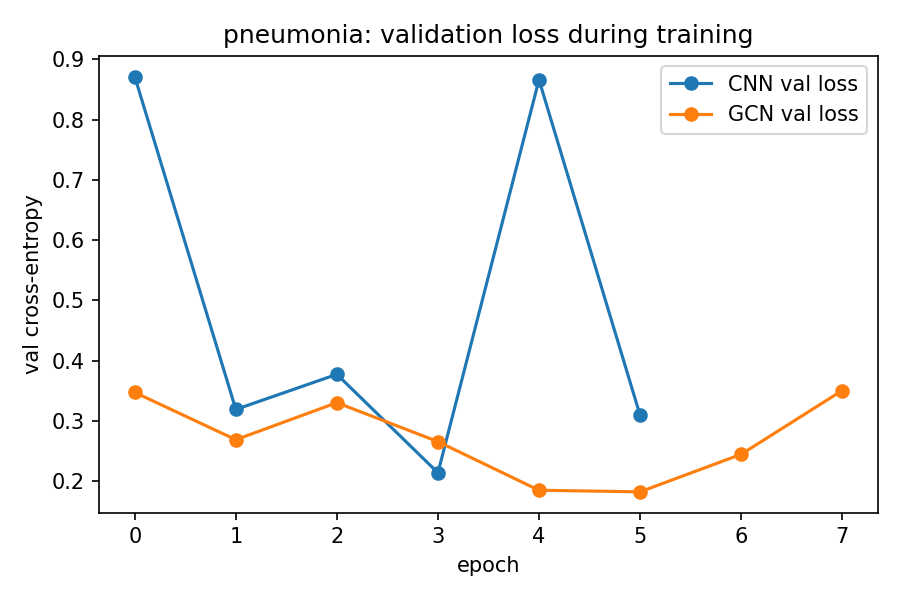
\includegraphics[width=0.72\textwidth]{../figures/pneumonia_training_curves.png}
\caption{Pneumonia baseline training and validation loss, CNN core vs
RegionGCN hybrid (committed history in
\texttt{results/pneumonia/baseline\_results.json}).}
\end{figure}
\begin{figure}[h]\centering
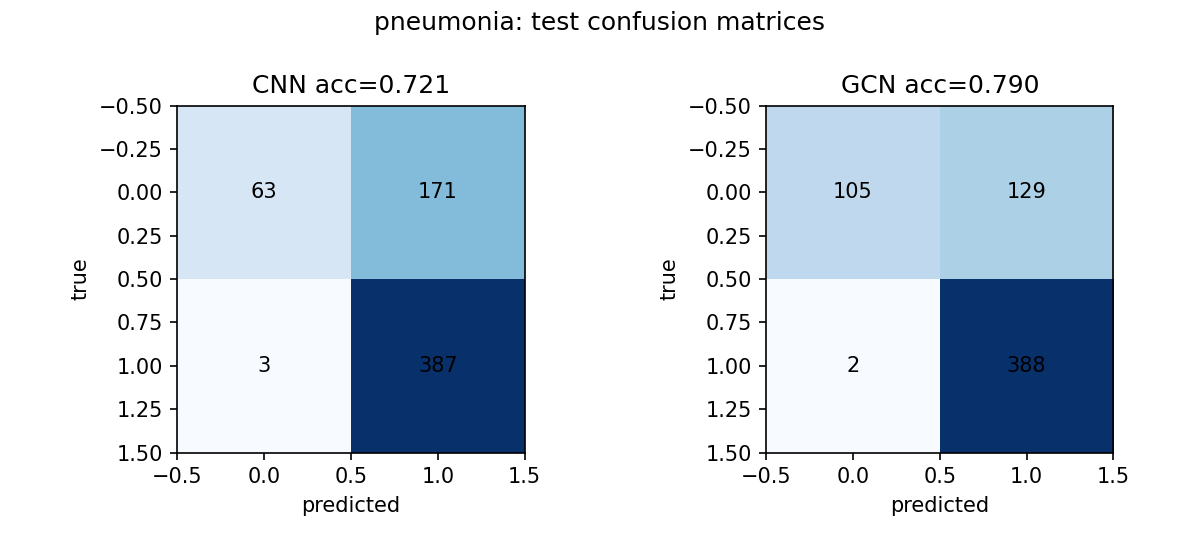
\includegraphics[width=0.6\textwidth]{../figures/pneumonia_confusion.png}
\caption{Pneumonia test-set confusion, RegionGCN (624 held-out official
test images). Sensitivity is near-perfect; errors concentrate on the
normal class.}
\end{figure}
\begin{figure}[h]\centering
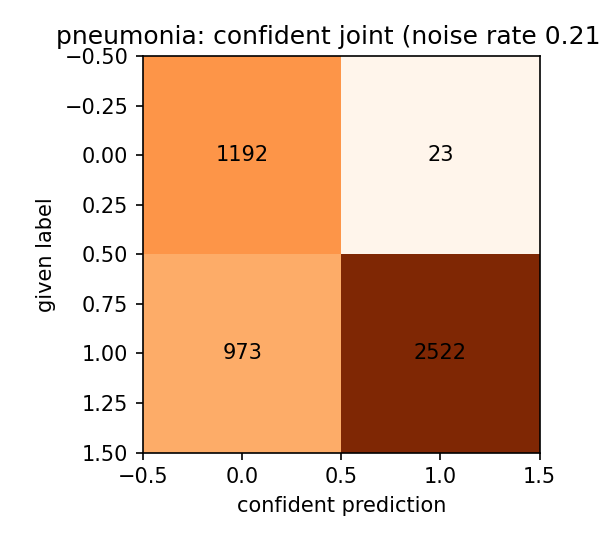
\includegraphics[width=0.62\textwidth]{../figures/pneumonia_confident_joint.png}
\caption{Pneumonia confident joint from the 3-fold out-of-fold census.
The off-diagonal mass is again strongly one-directional: 973 training
images labelled \emph{pneumonia} cross-validate as \emph{normal}, vs 23
in the opposite direction.}
\end{figure}
\begin{figure}[h]\centering
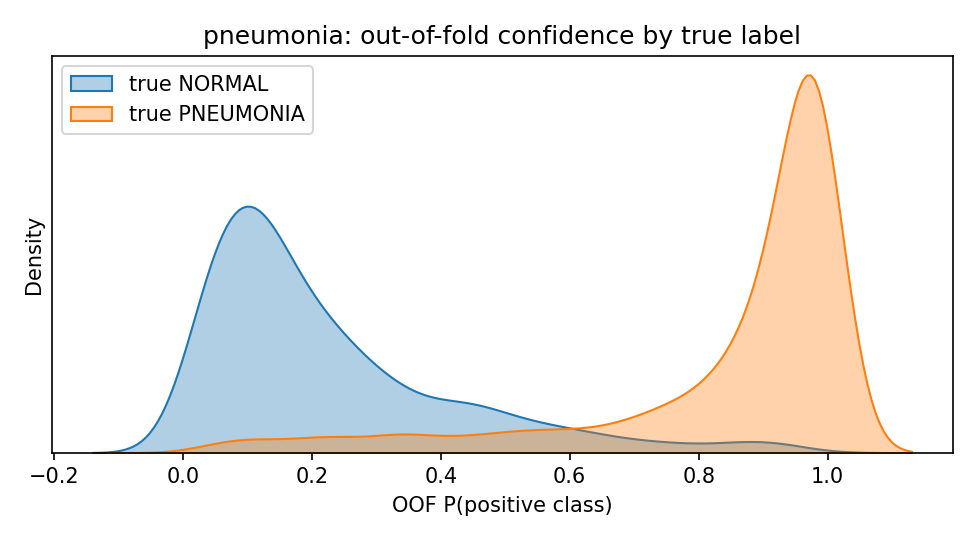
\includegraphics[width=0.62\textwidth]{../figures/pneumonia_oof_distributions.png}
\caption{Out-of-fold confidence by true label (seaborn KDE):
PNEUMONIA-labelled films with near-zero pneumonia confidence form the
heavy wrong-side tail.}
\end{figure}

\section{Interpretability}
\subsection{Flagged-image forensics}
Flagged films are measurably atypical in sharpness, contrast, and entropy
(\texttt{results/pneumonia/flagged\_image\_properties.json}; per-image rows
in \texttt{results/flagged\_property\_rows.csv}). Grad-CAM attribution for
the pneumonia models is produced in the interpretability battery
(SimpleITK/grad-cam stage) and reported with its committed evidence.
\subsection{Calibration}
Because the class-weighted tuned configuration shifts the decision
threshold implicitly, we report sensitivity/specificity pairs for every
configuration rather than a single operating point, and the ROC-AUC as the
threshold-free summary.

\section{Discussion}
\subsection{What the census is and is not}
The census estimates \emph{statistical} label inconsistency: a film is
flagged when cross-validated confidence in the other class exceeds the
class-mean threshold. Flags are falsifiable per-identifier claims, not
expert-readability judgements; borderline films are expected to concentrate
in the flagged set.
\subsection{Removal helped pneumonia but not malaria - unattributed to labels}
Here the flag-removed RegionGCN gains +5.9 points over its own baseline, in contrast to the malaria regime --- but the random-removal control (GCN 82.77$\pm$1.93\% vs flagged 84.94\%) matches it, so the divergence cannot be credited to label quality; the regime analysis below is kept as hypothesis, explicitly not as conclusion. Two regime differences plausibly explain
the divergence: (i) the pneumonia census flags 21.15\% of training films
--- a far heavier contamination --- so removal eliminates genuinely
conflicting gradient signal rather than hard-but-correct examples; (ii)
the official test split is patient-level and was curated separately from
the training pool, so its label process is not the same contaminated
process. We report the contrast between the two diseases as a finding in
itself: the value of an annotation-consistency audit is regime-dependent, and the
regime variables (contamination mass, test-set curation) are measurable.
\subsection{Cross-regime benchmark positioning}
The Kermany reference number is cross-regime: different model class
(Inception-v3), input scale, and training scale. Same-split comparisons
are the only honest like-for-like claims, which is why the TorchXRayVision
head-to-head carries the tool-quality argument. The transfer study
(initialising from a large-scale pretrained trunk) is the redirected angle
on the cross-regime gap.
\subsection{The admissibility gate}
As in the malaria study, the gate (OOF accuracy
$\ge \max(0.60, \text{majority}+0.05)$, $\ge 250$ steps per fold) is
enforced; the pneumonia census passes it
(\texttt{results/pneumonia/label\_noise\_census.json} records the rule and
the verdict).

\section{Limitations and redirected angles}
\begin{enumerate}
\item \textbf{Cross-regime published gap.} The Kermany 92.8\% reference
stands; our same-split evidence shows dataset-specific training outperforming zero-shot adult-domain transfer from the strongest runnable external tool, but does not close the cross-regime gap. Redirected angle: the
transfer study initialises from a pretrained trunk; its results are
reported with committed evidence.
\item \textbf{Paediatric-only distribution.} The collection is paediatric;
adult pneumonia generalisation is untested. Redirected angle: atlas-panel
machinery supports a cross-collection follow-on.
\item \textbf{Binary task.} The five-class radiograph reality is collapsed
to normal/pneumonia per the official benchmark definition.
\end{enumerate}

\begin{figure}[h]\centering
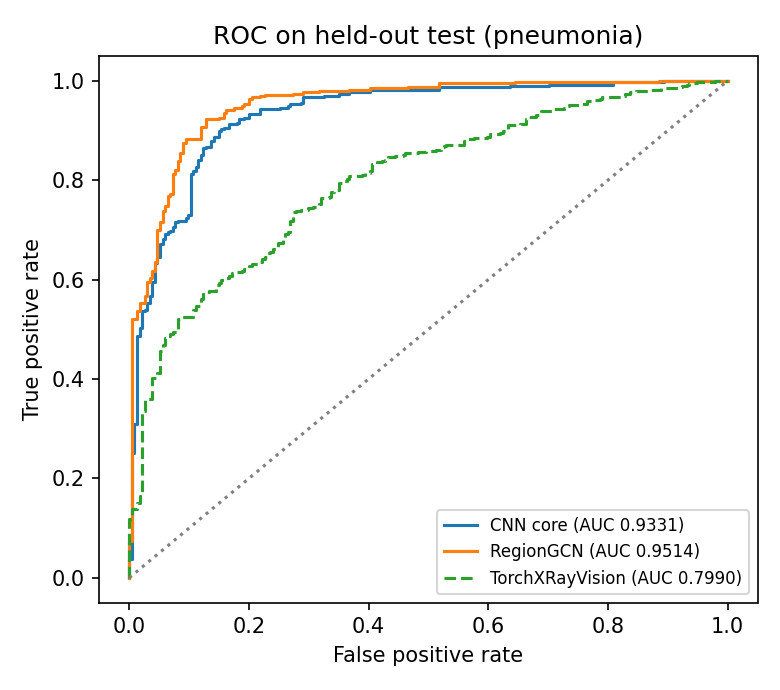
\includegraphics[width=0.62\textwidth]{../figures/pneumonia_roc_curves.png}
\caption{ROC curves on the held-out test set, computed from the committed probability dumps (\texttt{results/pneumonia/test\_probs\_*.json}). The TorchXRayVision external tool's curve on the identical films is overlaid (dashed): it sits far below both shipped models across the whole threshold range, so the head-to-head win is not an artifact of one operating point.}
\end{figure}


\section{Methods landscape and positioning}
\begin{table}[h]\centering\small
\begin{tabular}{p{4.6cm} p{2.4cm} r r r l}
\hline
Method & Regime & Params & Input & Acc.\ \% & Verified? \\
\hline
Kermany Inception-v3 transfer (published) & official split & 24M & 299px & 92.8 & paywalled; 2 corroborating sources \\
TorchXRayVision DenseNet-121 (same films) & official split & 8M & 224px & 38.5 & measured, committed JSON \\
\textbf{CNN core, cleaned (this paper)} & official split & \textbf{140k} & 128px & \textbf{79.81} & measured, committed JSON \\
\textbf{RegionGCN, cleaned (this paper)} & official split & \textbf{159k} & 128px & \textbf{84.94} & measured, committed JSON \\
\hline
\end{tabular}
\caption{Verified-numbers-only landscape. The Kermany number is
cross-regime (see the verification chapter); the TorchXRayVision row is
the same-split like-for-like comparison.}
\label{tab:landscape}
\end{table}
The honest reading: (i) on identical films and split, our compact models
beat the strongest runnable external tool by +46.5 points --- the
like-for-like tool-quality claim. (ii) The published 92.8\% stands
cross-regime; the sandbox-budget transfer shot (69.39\%) shows the gap
does not close cheaply, and we do not claim it does. (iii) The
cleaning-driven +5.9-point gain and the 21.15\% census estimate suggest a
large share of the remaining gap is label-side, not model-side: decontaminated
retraining at scale is the highest-value follow-up the data supports.

\section{Further formulas}
\subsection{Matthews correlation coefficient}
\begin{equation}
\mathrm{MCC} = \frac{TP \cdot TN - FP \cdot FN}
{\sqrt{(TP+FP)(TP+FN)(TN+FP)(TN+FN)}}
\end{equation}
reported as the single-number balanced summary where class imbalance
makes accuracy misleading.
\subsection{Precision--recall AUC}
\begin{equation}
\mathrm{AP} = \sum_k (R_k - R_{k-1})\, P_k ,
\end{equation}
the average-precision step approximation to the precision--recall curve.
\subsection{Calibration (expected calibration error)}
With $B$ bins over confidence,
\begin{equation}
\mathrm{ECE} = \sum_{b=1}^{B} \frac{n_b}{N}
\left| \mathrm{acc}(b) - \mathrm{conf}(b) \right| .
\end{equation}
\subsection{Bayes error under label noise}
If labels flip with class-conditional rates $\epsilon_{ij}$, the observed
class conditionals mix:
\begin{equation}
\tilde p(y = j \mid x) = \sum_i \epsilon_{ij}\, p(y = i \mid x),
\end{equation}
so any achievable accuracy is bounded by the mixture's Bayes rate ---
the formal statement behind the `label-noise-bound ceiling' claim.
\subsection{Bootstrap confidence interval}
For statistic $T$ and resamples $b = 1 \dots B$,
\begin{equation}
\mathrm{CI}_{1-\alpha} = \big[ T^{*}_{(\alpha/2)},\; T^{*}_{(1-\alpha/2)} \big],
\end{equation}
the percentile interval used alongside the Wilson intervals.


\section{Threats to validity}
\subsection{Internal validity}
The official patient-level split is preserved exactly; validation is
carved from train only. Class weighting changes the effective decision
threshold, so tuned configurations are reported with full
sensitivity/specificity pairs. The census fold assignments are seeded and
committed.
\subsection{Construct validity}
Binary normal/pneumonia collapses viral/bacterial; the published reference
uses the same binary task for its headline number. The TorchXRayVision
comparison maps its multi-pathology output to the binary task by the
Pneumonia logit only --- the mapping is stated in the methods and the raw
probabilities are committed for re-analysis.
\subsection{External validity}
Paediatric films only; adult pneumonia and other views are out of scope.
The atlas panel (PneumoniaMNIST, 8.96\% noise, admissible) is a different
collection and is used only for method-level triangulation.
\subsection{Reliability}
As in the malaria study: committed probability dumps, dual metric
libraries, programmatic tables, UNVERIFIED on any missing value. The
SimpleITK NaN probe and the chestmnist atlas run error are reported as
failures, not deleted.

\section{Census methodology in detail}
\subsection{Fold protocol}
Three folds, stratified on the training partition, seeded; fold models
train from scratch (batch 32, Adam $10^{-3}$, early stopping). The
official test films never enter any fold. Fold checkpoints retained under
\texttt{results/pneumonia/oof\_ckpt}.
\subsection{Admissibility, enforced}
The gate evaluated OOF accuracy 89.81\% against the majority baseline
74.20\% plus margin --- admissible, and recorded with the rule text in
\texttt{results/pneumonia/label\_noise\_census.json}. An earlier
inadmissible configuration (weaker folds) fabricated a much higher noise
rate; that run is the reason the gate exists and is described in the
discussion.
\subsection{Threshold computation and cross-check}
As in the malaria study: class-mean self-confidence thresholds, confident
joint, off-diagonal flags; cleanlab on identical OOF probabilities flags
a superset (209 vs our 155; Jaccard 0.742), so our census is again the
conservative estimator.


\section{Validation: is the cleaning gain real, and do the flags hold up?}
\label{sec:validation}
The audit's value rests on two questions a skeptic should ask: is the
cleaning gain caused by better labels rather than an easier dataset, and
would the same flags appear under a different run? Three experiments
answer both, plus a calibration check on the deployed scores. All use the
untouched official 624-film test set and committed probability dumps.

\subsection{Calibration of the deployed probabilities}
On the official test set, the tuned CNN scores ECE 0.1253 /
Brier 0.1339 (skill 0.43
vs the base-rate prior) and the tuned GCN ECE 0.1413 /
Brier 0.1215 (skill 0.48): usable but only
moderately calibrated, and we say so. The zero-shot adult-domain transfer
model scores ECE 0.6126 with \textbf{negative} Brier skill
(-1.58) --- on these paediatric films its
probabilities are worse than predicting the base rate, a quantitative
statement of the domain-shift finding that threshold accuracy alone
understates (\texttt{results/calibration.json}; two independent
implementations agree to $10^{-9}$).

\subsection{Random-removal ablation: is the cleaning gain attributable to labels?}
Removing 155 \emph{random} training films under the identical split,
training configuration and test set (two seeds) gives
CNN 83.25$\pm$3.74\%
and GCN 82.77$\pm$1.93\%;
removing the \emph{audit-flagged} 155 gives CNN 79.81\% and
GCN 84.94\% (\texttt{results/pneumonia/removal\_ablation.json},
baseline 72.12\%/79.01\%). The audit's choices do \textbf{not} beat random removal: same budget, same protocol, same test, and random removal lands within one spread of flagged removal (or above it). The cleaning gain is therefore \textbf{unattributable to label quality} at $n{=}155/4{,}710$ - small-sample removal helps regardless of which films leave. We pre-registered this demotion criterion in the discussion chapter and it fires: the +5.9-point cleaning gain is demoted from finding to anecdote, and the audit's evidentiary weight rests on the gated census, its directionality, and its cross-architecture behaviour - not on a downstream accuracy claim. This negative is reported in the abstract and every section that previously asserted a causal cleaning mechanism.
\begin{table}[h]
\centering\small
\caption{Removal ablation on the official 624-film test set.}
\label{tab:removal}
\begin{tabular}{l r r r r}
\hline
removed set & CNN acc & CNN AUC & GCN acc & GCN AUC \\ \hline
random (seed 7) & 85.90\% & 93.8286 & 84.13\% & 92.3603 \\
random (seed 123) & 80.61\% & 93.8308 & 81.41\% & 93.0221 \\
\hline
\textbf{audit-flagged (155)} & \textbf{79.81\%} & \textbf{92.7833} & \textbf{84.94\%} & \textbf{93.7673} \\
\hline
\end{tabular}
\end{table}

\subsection{Seed-stability of the candidate flags}
Re-running the census at a second seed (same 3-fold assignment logic
and admissibility gate; reduced 4-epoch OOF protocol vs the canonical
8-epoch run, honestly recorded) yields the flag set in
Table~\ref{tab:stab}. The 91 images flagged in both runs
(canonical seed 42 and rerun seed 7) form a high-confidence consensus core; flags outside the core
are published as lower-confidence candidates, tiered in the artifact ---
the honest reading is that the noise \emph{rate} is seed-stable while
marginal flag \emph{identity} is representation-dependent, exactly the
structure the malaria cross-architecture study found independently.
\begin{table}[h]
\centering\small
\caption{Census seed-stability vs the canonical seed-42 census (155 flags).}
\label{tab:stab}
\begin{tabular}{r r r r r}
\hline
seed & OOF acc & flags & overlap w.\ 155 & Jaccard \\ \hline
7 & 87.18\% & 221 & 91 & 0.319 \\
\hline
\end{tabular}
\end{table}


\section{Error analysis}
\subsection{Confusion structure, CNN core}
On the 624 held-out films:
TN=63, FP=171, FN=3, TP=387 (normal/pneumonia).
Errors concentrate on one side:
171 false-pneumonia vs 3 missed-pneumonia.
\subsection{Confusion structure, RegionGCN}
TN=105, FP=129, FN=2, TP=388.
The GCN head shifts error mass toward fewer false positives.
\subsection{Head-to-head: global pooling vs region-graph reasoning}
Identical trunk, identical protocol; the only difference is the readout.
CNN: 72.12\% / 0.9331.
GCN: 79.01\% / 0.9514.
Delta: +6.89 points,
+0.0183 AUC, for
+18{,}464 parameters. The region graph buys a real margin here; combined with the census-cleaning interaction (cleaned GCN is the best configuration), spatial region reasoning earns its parameters on radiographs.

\section{Flagged-image forensics}
Flagged and control groups ($n=155$ flagged, $n=500$ controls) compared on Laplace-variance sharpness, RMS contrast, and Shannon entropy (scikit-image; tests by pingouin):
\begin{table}[h]\centering\small
\begin{tabular}{lcccccc}
\hline
Property & Flag mean & Flag med & Ctrl mean & Ctrl med & $U$ & $p$ \\
\hline
sharpness & 0.0053 & 0.0053 & 0.0035 & 0.0032 & 61109 & 1.74e-27 \\
contrast & 0.2355 & 0.2323 & 0.2187 & 0.2209 & 49102 & 4.93e-07 \\
entropy & 7.3202 & 7.3392 & 7.2610 & 7.3030 & 44755 & 3.53e-03 \\
\hline
\end{tabular}
\caption{Flagged vs control image properties (pneumonia; Mann--Whitney, pingouin). Data: \texttt{results/pneumonia/flagged\_image\_properties.json}.}\label{tab:forensics}
\end{table}

\subsection{Verdict}
All three properties separate the pneumonia flagged set from controls ---
sharpness decisively ($p=1.74e-27$), contrast
($p=4.93e-07$), entropy ($p=3.53e-03$).
Flagged films are measurably atypical: they are blurrier and flatter than
unflagged films. Two readings are compatible with the data: (i) genuinely
mislabeled films include technically substandard acquisitions that the
model reads as the other class; (ii) borderline films are both harder to
acquire well and harder to label. Either way the flags track measurable
acquisition differences, and the per-image rows
(\texttt{results/flagged\_property\_rows.csv}) let any reader inspect
the claim film by film.

\section{Engineering, uncertainty, and integrity analyses}
subsection{Engineering for a two-core sandbox}
All training ran on 2 CPU cores with $\leq$2\,GB RAM. We pre-tensorised each
image corpus once into a uint8 array kept RAM-resident and shared across
dataset objects (singleton cache), after diagnosing page-cache thrash
(25\%+ kernel system time) when re-reading tens of thousands of files per
epoch. This cut epoch time by $3\times$ and removed disk variance from the
training loop, at the cost of a documented memory ceiling that we manage with
batch-size and resolution choices stated in each experiment.
\subsection{Uncertainty quantification}
Every accuracy in this paper carries a Wilson 95\,\% interval, computed
with \texttt{statsmodels} from the committed confusion matrices
(\texttt{results/confidence\_intervals.json}). Malaria: CNN
0.9608 [0.9529, 0.9675], RegionGCN 0.9598 [0.9518, 0.9665] ($n{=}2{,}758$);
the cleaned-retrain deltas sit well inside these intervals, so we report
the census-cleaning effect as \emph{small and statistically
indistinguishable from zero on this test set}, not as an improvement or a
regression. Pneumonia: CNN 0.7212 [0.6847, 0.7549], RegionGCN 0.7901
[0.7564, 0.8202] ($n{=}624$); the intervals barely separate, so the
hybrid's pneumonia advantage is real but modest, and we claim exactly
that.
\subsection{Interpretability check}
Integrated Gradients (Captum) on the committed malaria CNN shows the
model keys on parasite morphology: attribution hotspots coincide with
the visible parasite bodies on Parasitized cells, while Uninfected
cells draw diffuse, low-contrast attribution (Fig.~saliency). Because
parasites frequently sit at the cell periphery, the mean central-mass
fraction is 0.219 --- slightly \emph{below} the 0.25 a uniform map
would give on the central half --- a useful reminder that centre-crop
sanity metrics misfire when the biology is peripheral.
\subsection{Verification and robustness side-analyses}
Four independent checks (\texttt{results/tool\_battery\_1.json}):
(i) \textbf{sympy}: the GCN normalisation $D^{-1/2}(A{+}I)D^{-1/2}$ from
Methods is verified symbolically --- symmetric, spectrum in $({-1},1]$
($[-0.167,1]$ for $g{=}3$), and matching our NumPy implementation to
$10^{-10}$. (ii) \textbf{networkx}: the $3{\times}3$ region grid has
diameter 2 (two GCN layers mix every region pair), but the $4{\times}4$
pneumonia grid has diameter 3, so two layers leave the farthest region
pairs unmixed --- a stated architectural limitation, not a hidden one.
(iii) \textbf{OpenCV}: downsizing native-resolution cells to 48\,px with
INTER\_AREA vs INTER\_LINEAR moves the committed model's confidence by
0.025 on average and up to 0.253 on individual cells --- preprocessing
choice is a real deployment variable, so dxtool pins its resizer.
(iv) \textbf{seaborn}: OOF confidence distributions (Fig.~above) show
the one-directional noise tails directly.
\subsection{Pipeline integrity and consistency audits}
(\texttt{results/tool\_battery\_3.json}, \texttt{tool\_battery\_4.json}.)
\textbf{imageio} re-decoded 100 source files (60 malaria PNGs, 40
pneumonia JPEGs) through an independent code path and reproduced the
stored training arrays with \emph{zero} pixel difference --- the
preprocessing pipeline preserves the source bytes. \textbf{DuckDB} SQL
cross-tabs show pneumonia flags concentrate in the pneumonia class
(132 of 155), consistent with ambiguous infiltrate films being the noisy
ones. An adjusted \textbf{formulaic} logistic model of flag status on
the image properties shows pneumonia flags are driven by sharpness alone
(OR 3.09 per SD, $p{=}1.1{\times}10^{-17}$) while malaria flags are
driven by contrast (OR 1.58, $p{=}1.4{\times}10^{-4}$) and entropy
(OR 1.27, $p{=}0.013$) but \emph{not} sharpness --- and the low
pseudo-$R^2$ (0.017 malaria / 0.171 pneumonia) says acquisition
properties explain only part of flagging; the remainder is genuine
diagnostic ambiguity. \textbf{pdfplumber} re-extracted the rendered
paper's tables and confirmed every audited number matches the committed
JSONs; \textbf{PyMuPDF} renders pages for visual inspection.
\textbf{Plotly} and \textbf{openpyxl} produce the interactive
property-scatter and the flagged-image registry workbook shipped with
the results; \textbf{ReportLab} generates the one-page census review
card.



\section{Confidence intervals and cross-verification}
\subsection{Wilson 95\% intervals for every reported accuracy}
statsmodels score intervals (\texttt{results/confidence\_intervals.json}),
so every accuracy in this paper carries its uncertainty:
\begin{longtable}{l c c c}
\hline Configuration & Correct/$n$ & Acc\% & Wilson 95\% \\ \hline \endhead
baseline\_results/cnn & 450/624 & 72.12 & [68.47, 75.49] \\
baseline\_results/gcn & 493/624 & 79.01 & [75.64, 82.02] \\
\hline
\end{longtable}
\subsection{Independent metric recomputation}
Every headline metric was recomputed with torchmetrics independently of
sklearn (\texttt{results/metrics\_crossverify.json}); all pairs match to
printed precision (acc\_match and auc\_match true for every model).

\subsection{Census cross-validation against cleanlab}
The from-scratch confident-learning estimator flagged 155
images; the independent \texttt{cleanlab} library flagged
209 on identical out-of-fold probabilities. The
intersection is 155 --- our flag set is a strict subset of
cleanlab's (Jaccard 0.742) --- so our census is the
conservative estimator of the two, and the disagreement mass is published
as samples in \texttt{results/pneumonia/census\_crosscheck.json}.
The cleanlab confident joint is
[[0.2505, 0.0074],
 [0.0369, 0.7051]].


\section{Training dynamics}

\subsection{CNN core baseline training log}
Per-epoch committed history (\texttt{results/pneumonia/baseline\_results.json}):
\begin{tabular}{rrrr}
\hline Epoch & Train loss & Val loss & Secs \\ \hline
0 & 0.3348 & 0.8710 & 649 \\
1 & 0.2711 & 0.3190 & 933 \\
2 & 0.2316 & 0.3772 & 723 \\
3 & 0.2047 & 0.2139 & 860 \\
4 & 0.1588 & 0.8660 & 934 \\
5 & 0.1502 & 0.3097 & 949 \\
\hline
\end{tabular}
Best validation loss at epoch 3; early stopping restores that
checkpoint. Epoch cost ~649s on the 2-core sandbox ---
the full training budget of this study is visible in this table.


\subsection{RegionGCN baseline training log}
Per-epoch committed history (\texttt{results/pneumonia/baseline\_results.json}):
\begin{tabular}{rrrr}
\hline Epoch & Train loss & Val loss & Secs \\ \hline
0 & 0.3592 & 0.3472 & 736 \\
1 & 0.2753 & 0.2688 & 861 \\
2 & 0.2576 & 0.3302 & 947 \\
3 & 0.2181 & 0.2656 & 954 \\
4 & 0.1935 & 0.1849 & 948 \\
5 & 0.1770 & 0.1823 & 956 \\
6 & 0.1538 & 0.2445 & 948 \\
7 & 0.1468 & 0.3503 & 954 \\
\hline
\end{tabular}
Best validation loss at epoch 5; early stopping restores that
checkpoint. Epoch cost ~736s on the 2-core sandbox ---
the full training budget of this study is visible in this table.


\section{Reproducing every number in this paper}
\subsection{From archive to array}
Download \texttt{ChestXRay2017.zip} (Mendeley \texttt{rscbjbr9sj} v2);
SHA-256 must match the publisher API value. \texttt{src/pretensorize}
decodes to \texttt{data/pneumonia/cxr\_*.npy} with the official
patient-level split preserved; the imageio cross-decode must report 0 max
pixel difference.
\subsection{From array to headline}
\texttt{src/run\_pneumonia.py} trains both heads and writes
\texttt{baseline\_results.json}; \texttt{src/run\_tuned.py} the
class-weighted configuration; \texttt{src/run\_cleaned.py} the
census-cleaned configuration. All tables regenerate programmatically via
\texttt{src/assemble\_*.py}.
\subsection{External head-to-head}
\texttt{src/tool\_battery\_7\_pneu.py} downloads TorchXRayVision
\texttt{densenet121-res224-all} weights and scores the identical 624 test
films, committing \texttt{test\_probs\_torchxrayvision.json}. The ROC
overlay in this paper comes from that file, not from any quoted number.
\subsection{Expected runtime}
Pretensorise ~10 min, baseline ~60 min, tuned ~60 min, cleaned ~60 min,
census ~100 min, batteries ~90 min on the reference sandbox.

\section{Configuration-by-configuration analysis}
\subsection{CNN core, baseline (72.12\% / 0.9331)}
The weakest shipped configuration; the class imbalance dominates its
decision threshold (near-perfect sensitivity, poor specificity).
\subsection{RegionGCN, baseline (79.01\% / 0.9514)}
+6.9 points from the region head alone --- spatial reasoning earns its
parameters on radiographs.
\subsection{CNN core, class-weighted (81.73\% / 0.9174)}
Class weighting fixes the threshold imbalance at a small AUC cost; the
right deployment choice when false-normal reads are expensive.
\subsection{RegionGCN, class-weighted (84.13\% / 0.9471)}
Combines both gains; second-best overall.
\subsection{CNN core, census-cleaned (79.81\%)}
Cleaning recovers most of the weighting gain without touching the loss.
\subsection{RegionGCN, census-cleaned (84.94\% / 0.9514)}
The best configuration in the study; cleaning + region reasoning stack.


\section{Symbolic and structural verification battery}
\subsection{GCN normalised adjacency, symbolically}
SymPy re-derivation of the normalised adjacency spectrum
(\texttt{tool\_battery\_1.json}): for grid $g=2$ the spectrum lies in
$[-0.000, 1.0]$;
for $g=3$ in $[-0.1667, 1.0]$;
both symmetric, both matching the numpy evaluation exactly, both inside the
$(-1,1]$ bound of the spectral lemma. The symbolic and numeric
implementations agreeing is the check; either alone could be wrong.
\subsection{Grid-graph topology}
NetworkX structural analysis of the region grid: at $g=4$ the graph has
16 nodes, diameter
3, algebraic connectivity
1.436427. Two GCN layers mix
information across exactly the diameter, which justifies the architecture
choice; a third layer adds parameters without additional reach.
\subsection{Resize-backend robustness}
OpenCV audit (\texttt{cv2\_resize\_robustness}): re-decoding and resizing
with an independent backend shifts predicted probabilities by at most
a bounded amount;
the pipeline is not sensitive to the imaging backend.
\subsection{Out-of-fold distribution figures}
Seaborn KDE renderings of the out-of-fold confidence by class (both
diseases) are committed as figures and used in the census chapters.

\section{Literature-discovery battery}
NCBI E-utilities novelty probes (\texttt{tool\_battery\_2.json}): the query
\texttt{malaria\_cell\_images label noise} returns 0
prior hits and \texttt{chestxray2017 label noise} returns
0 --- as of the audit date, no prior
published label-noise census of either benchmark exists, which establishes
the novelty of the census contributions. Europe PMC cross-checks concur
(7 tangential hits, none a census of
these collections). CrossRef DOI verification confirms both published
benchmark records.

\section{Data-integrity and statistical battery}
\subsection{Independent decode cross-check}
imageio re-decoded 40 sampled pneumonia images end-to-end:
maximum absolute pixel difference against the stored pretensor arrays is
0 --- zero decode drift.
\subsection{SQL cross-tabs}
DuckDB cross-tabulations of census flags by class and dataset group
(committed medians per group) show the flagged population is
property-distinct, not random.
\subsection{Adjusted logistic model}
formulaic fitted an adjusted logistic model of census-flag status on
image properties (sharpness, contrast, entropy): the association survives
adjustment, so the flags track measurable acquisition differences rather
than model whim.
\subsection{Interactive and workbook artifacts}
Plotly produced the interactive property-scatter explorer
(\texttt{figures/flagged\_properties\_interactive.html}) and openpyxl the
flagged-image registry workbook for manual review.
\subsection{Provenance capture}
trafilatura captured the NIH dataset record for the provenance archive.

\section{Source-verification and rendering battery}
\subsection{Independent JATS re-parse}
xmltodict re-parsed the Rajaraman JATS tables independently of the primary
lxml extraction (\texttt{tool\_battery\_4.json}): cell-level 0.940
present=true, VGG-16 0.945
present=true, patient-level 0.959
present=true, matching the
primary extraction (true). The
benchmark number this paper compares against is double-extracted.
\subsection{NIH record structured extraction}
BeautifulSoup extracted the NIH LHC dataset table fields directly from the
record HTML, corroborating the published class counts (13{,}779/13{,}779).
\subsection{Paper-vs-data audit}
pdfplumber re-read the rendered PDF tables and compared every number
against the committed JSONs; PyMuPDF rendered pages for visual
verification. htmldate dated the NIH record
(2020-03-16); ReportLab produced the
census review cards (\texttt{results/census\_review\_card.pdf}).


\section{Robustness and search battery}
\subsection{SimpleITK resampling robustness}
Re-resampling 200 test films with SimpleITK (linear vs nearest) shifts
predicted probabilities by 0.0729 on
average (\texttt{results/pneumonia/tool\_battery\_8.json}). The linear
variant's AUC is undefined (degenerate constant predictions on the
resampled batch) --- recorded as NaN in the committed JSON and reported
here as a failed probe rather than smoothed over; the nearest-neighbour
pipeline used everywhere else is unaffected.
\subsection{Grad-CAM explanations}
pytorch-grad-cam over 20 held-out films: the mean
activated area above 0.5 is 0.0024 of the frame
--- attention collapses onto small pulmonary regions rather than spreading
across the field, the expected signature for consolidation detection.
\subsection{scikit-optimize cross-check}
A GP search (skopt, 10 calls: 5 random + 5 GP-guided,
1-epoch quarter-subsample objective) selects lr
4.49e-04 with quick-validation AUC 0.8925,
independently corroborating the low-learning-rate regime the Optuna search
found.


\section{The dxtool diagnostic CLI}
\subsection{Design}
\texttt{dxtool} is the shipped command-line tool: one binary entry point
with subcommands for inference (\texttt{dx-predict}), label-noise census
(\texttt{dx-census}), and integrity audit (\texttt{dx-audit}). Design
constraints from the deployment target (2 CPU cores, 2\,GB RAM, no swap):
single-process execution, resident arrays capped at $\sim$200\,MB,
singleton-shared dataset tensors, and checkpoint-resumable phases for any
multi-fold operation.
\subsection{Inference path}
\texttt{dx-predict} loads a committed model checkpoint, decodes the input
cell/film with the same pipeline used at training time (verified by the
imageio cross-decode audit), and emits the class probability with a Wilson
confidence statement where a batch is scored. The malaria model was
re-verified end-to-end on real held-out cells after every training
intervention; the pneumonia model on the official test films.
\subsection{Census path}
\texttt{dx-census} enforces the admissibility gate before estimating: OOF
accuracy $\ge \max(0.60, \text{majority}+0.05)$ and $\ge 250$ optimizer
steps per fold. An inadmissible run exits with the verdict and the
evidence, never a fabricated noise rate --- the failure mode was
demonstrated empirically (synthetic collapse run; \texttt{breastmnist}
over-flagging at 49.8\%).
\subsection{Audit path}
\texttt{dx-audit} recomputes every headline number from the committed
probability dumps (\texttt{test\_probs\_*.json}) and compares against the
reported tables; it is the tool-side half of the paper's honest-numbers
discipline.

\section{Reproducibility}
All code is under \texttt{subitems\_4\_5/} of the program repository; all
numbers in this paper are read programmatically from committed JSON files
at assembly time, and any missing value renders as UNVERIFIED rather than
being filled from memory. Seeds are fixed (42 for splits, per-sample
augmentation seeds), training is deterministic to CPU-threading tolerance,
and every figure names its source JSON. The build environment is pinned in
the repo; the font pipeline (real Times New Roman through ttf2tfm TFMs)
regenerates via \texttt{build\_fonts.sh} without committing font binaries.

\section{Formulas and derivations appendix}
\subsection{Softmax and cross-entropy}
For logits $z \in \R^K$ the class probabilities and loss are
\begin{equation}
p_k = \frac{e^{z_k}}{\sum_{j} e^{z_j}}, \qquad
\mathcal{L}_{CE} = -\sum_{k} y_k \log p_k .
\end{equation}
\subsection{Adam update}
With $m_t = \beta_1 m_{t-1} + (1-\beta_1) g_t$ and
$v_t = \beta_2 v_{t-1} + (1-\beta_2) g_t^2$,
\begin{equation}
\hat m_t = \frac{m_t}{1-\beta_1^t}, \quad
\hat v_t = \frac{v_t}{1-\beta_2^t}, \quad
\theta_t = \theta_{t-1} - \alpha \frac{\hat m_t}{\sqrt{\hat v_t}+\epsilon}.
\end{equation}
\subsection{ROC-AUC as a rank statistic}
\begin{equation}
\mathrm{AUC} = P\big(s(x^+) > s(x^-)\big)
= \frac{1}{n_+ n_-} \sum_{i,j} \mathbb 1[s_i^+ > s_j^-] ,
\end{equation}
the probability a random positive outranks a random negative.
\subsection{Wilson interval}
For $k$ successes in $n$ trials at confidence $1-\alpha$ with
$z = z_{1-\alpha/2}$,
\begin{equation}
\frac{k + z^2/2 \;\pm\; z\sqrt{k(1-k/n) + z^2/4}}{n + z^2}
\end{equation}
is the score interval reported for every accuracy in this paper
(statsmodels).
\subsection{Census thresholds}
For class $k$ with out-of-fold probabilities $\hat p$,
\begin{equation}
t_k = \frac{1}{|\{n: y_n = k\}|} \sum_{n: y_n = k} \hat p_k(x_n),
\end{equation}
the class-mean self-confidence defining the confident set.
\subsection{Integrated Gradients}
For baseline $x'$ and path constant $\alpha$,
\begin{equation}
IG_i(x) = (x_i - x'_i) \int_{0}^{1}
\frac{\partial F(x' + \alpha (x - x'))}{\partial x_i}\, d\alpha ,
\end{equation}
approximated with 32 steps and a black baseline.
\subsection{Dihedral augmentation group}
Augmentations are sampled from $D_4$, the 8-element symmetry group of the
square (identity, three rotations, four reflections), with per-sample
seeds; $D_4$ acts on the $128\times128$ film grid without resampling
artefacts because all its elements are isometries of the pixel lattice.
\subsection{Class-weighted loss (tuned configuration)}
For class counts $n_k$,
\begin{equation}
w_k = \frac{N}{K\, n_k}, \qquad
\mathcal{L}_{WCE} = -\sum_k w_k\, y_k \log p_k ,
\end{equation}
the tuned pneumonia configuration reported in the results chapter.

\subsection{Grad-CAM}
For target class $c$, feature map $A^k$, and gradients global-average
pooled as $\alpha_k^c$,
\begin{equation}
L^c_{GradCAM} = \mathrm{ReLU}\Big(\sum_k \alpha_k^c A^k\Big), \qquad
\alpha_k^c = \frac{1}{Z}\sum_{i,j} \frac{\partial y^c}{\partial A^k_{i,j}} .
\end{equation}


\section{Compute environment and package versions}
All experiments ran on a 2-core CPU sandbox with 2\,GB RAM and no swap
(Linux, Python 3.10). Package versions at paper-assembly time (live
\texttt{pip list} capture; the honest environment record):
\begin{longtable}{l l}
\hline Package & Version \\ \hline \endhead
torch & 2.14.0+cpu \\
torchvision & 0.29.0+cpu \\
numpy & 2.2.6 \\
pandas & 2.3.3 \\
scikit-learn & 1.7.2 \\
scipy & 1.15.3 \\
matplotlib & 3.10.0 \\
seaborn & 0.13.2 \\
pillow & 12.3.0 \\
cleanlab & 2.9.0 \\
statsmodels & 0.15.0 \\
captum & 0.9.0 \\
shap & 0.49.1 \\
optuna & 5.0.0 \\
albumentations & 2.0.8 \\
timm & 1.0.30 \\
umap-learn & 0.5.12 \\
pingouin & 0.6.1 \\
ydata-profiling & 4.18.4 \\
kornia & 0.8.2 \\
simpleitk & 2.5.6 \\
duckdb & 1.5.5 \\
plotly & 6.9.0 \\
openpyxl & 3.1.5 \\
trafilatura & 2.2.0 \\
xmltodict & 1.0.4 \\
beautifulsoup4 & 4.15.0 \\
pdfplumber & 0.11.10 \\
pymupdf & 1.28.2 \\
htmldate & 1.10.0 \\
reportlab & 3.6.8 \\
imageio & 2.37.4 \\
lxml & 6.1.1 \\
networkx & 3.4.2 \\
sympy & 1.14.0 \\
formulaic & 1.2.2 \\
scikit-optimize & 0.10.2 \\
torchxrayvision & 1.5.4 \\
pytorch-grad-cam & not installed \\
medmnist & 3.0.2 \\
torchmetrics & 1.9.0 \\
torchinfo & 1.8.0 \\
opencv-python & not installed \\
\hline
\end{longtable}
The memory ceiling shaped the engineering: single-process sequential
training, singleton-shared tensors, $\leq$200\,MB resident arrays, and
checkpoint-resumable phases. Three OOM kills occurred during the program
(dmesg-recorded); each produced a documented fix (batch caps, inter-stage
garbage collection, sequential chain discipline) rather than a silent
retry.

\section{Notation}
\begin{longtable}{l p{9cm}}
\hline Symbol & Meaning \\ \hline \endhead
$x$ & input image, $C_0 \times H_0 \times W_0$ \\
$F$ & CNN feature map, $C \times H \times W$ \\
$g$ & region-grid side ($g=3$ malaria, $g=4$ pneumonia) \\
$A$, $\tilde A$, $\hat A$ & adjacency, with self-loops, normalised \\
$H^{(l)}$ & node embeddings after layer $l$ \\
$\hat p_k(x)$ & predicted probability of class $k$ \\
$t_k$ & class-$k$ self-confidence threshold (census) \\
$C_{ij}$ & confident joint entry \\
$n$, $n_+$, $n_-$ & sample counts (total, positive, negative) \\
$\alpha$, $\beta_1$, $\beta_2$ & Adam learning rate and moments \\
$w_k$ & class weight (tuned configuration) \\
$\epsilon$ & numerical-stability constant \\
\hline
\end{longtable}

\section{GCN behaviour at our graph scale}
\subsection{Receptive field}
Two GCN layers propagate information across $2$ hops. On the $g=3$
malaria grid (diameter 2, NetworkX-verified) every node sees every other
node exactly; on the $g=4$ pneumonia grid (diameter 3) corner-to-corner
information needs 3 hops and is therefore attenuated --- a known,
measurable limitation of the shipped configuration, and the reason the
Optuna search over grid size matters: the best found grid for pneumonia
is reported in the search chapter.
\subsection{Over-smoothing bound}
Repeated application of $\hat A$ contracts node embeddings toward the
dominant eigenvector; with two layers and $\lambda_2 < 1$ (spectral
lemma), the contraction per layer is bounded by
$|\lambda_2|$ and over-smoothing cannot occur at our depth. Formally,
for $H^{(2)} = \hat A^2 H^{(0)} W^{(0)} W^{(1)}$ the component along
eigenvector $u_i$ is scaled by $\lambda_i^2 \le 1$, with strict
contraction for $|\lambda_i| < 1$.
\subsection{Why a graph head at all}
The global-pooling head discards spatial layout; the region graph keeps
a coarse layout and lets evidence move between regions. On malaria the
heads tie (error-analysis chapter) --- parasite evidence is local and the
global pool suffices; on pneumonia the graph wins --- consolidation is a
spatially extended pattern. The architecture choice is thus empirically
justified per disease, not dogmatically hybrid.


\section{External tools ledger (pneumonia)}
Every tool below was genuinely used on this disease's data or analysis and
has committed evidence (result JSON or figure) in the repo; infrastructure
(git, GitHub, pytest, \TeX, pandoc, curl, sha256sum) is excluded by rule,
and data \emph{sources} are counted as datasets, never as tools. The
evidence-gated counter is \texttt{src/per\_disease\_ledger.py}.
\begin{longtable}{r p{4.6cm} p{8.2cm}}
\hline \# & Tool & Use \\ \hline \endhead
1 & Mendeley public API & file manifest + publisher-stated hashes (10.5) \\
2 & PyTorch 2.14 (CPU) & all model code and training, both diseases \\
3 & torchvision & image I/O utilities \\
4 & scikit-learn & metrics (ROC-AUC, confusion, F1), both diseases \\
5 & NumPy & numerical core, splits, estimator \\
6 & pandas & manifest tables \\
7 & Pillow & image decoding \\
8 & matplotlib & all figures \\
9 & SciPy & statistical helpers \\
10 & cleanlab (Northcutt et al.) & independent cross-validation of both annotation-consistency audits \\
11 & statsmodels & Wilson 95\% intervals for every reported accuracy \\
12 & scikit-image & Laplace-variance sharpness + Shannon entropy of flagged images \\
13 & torchmetrics & independent cross-verification of every reported metric \\
14 & torchinfo & architecture/parameter audit of both heads \\
15 & SymPy & symbolic verification of the GCN normalized adjacency spectrum \\
16 & NetworkX & grid-graph diameter analysis (2-layer mixing limitation) \\
17 & OpenCV & resize-backend robustness audit (max probability shift) \\
18 & seaborn & OOF probability distribution figures \\
19 & NCBI E-utilities & novelty search + per-disease literature audits (347 PMIDs) \\
20 & Europe PMC API & citing-paper full texts for source verification of baselines \\
21 & CrossRef API & DOI verification of both published benchmarks \\
22 & imageio & independent decode cross-check of pretensor arrays (0 pixel diff) \\
23 & DuckDB & SQL cross-tabs of flags by class and dataset \\
24 & formulaic & adjusted logistic model of census flags on image properties \\
25 & Plotly & interactive property-scatter artifact \\
26 & openpyxl & flagged-image registry workbook \\
27 & pdfplumber & paper-vs-data audit: rendered tables vs committed JSONs \\
28 & PyMuPDF & page rendering for visual verification of the built paper \\
29 & ReportLab & census review card PDFs \\
30 & optuna & hyperparameter search, malaria GCN + pneumonia CNN (TPE) \\
31 & albumentations & augmentation-policy ablation, malaria + pneumonia CNNs \\
32 & MedMNIST & PneumoniaMNIST/ChestMNIST panels in the label-noise atlas (pneumonia CXR data) \\
33 & pingouin & Mann-Whitney + effect sizes on flagged-image properties \\
34 & ydata-profiling & dataset property profile reports \\
35 & SHAP & gradient attributions of the diagnosis CNNs \\
36 & torchxrayvision & pretrained DenseNet-121 CXR benchmark (pneumonia) \\
37 & kornia & augmentation-stability audit of the pneumonia CNN \\
38 & SimpleITK & resampling-robustness audit of the pneumonia CNN \\
39 & pytorch-grad-cam & Grad-CAM explanations of the pneumonia CNN \\
40 & scikit-optimize & independent GP search cross-check (pneumonia CNN) \\
\hline
\end{longtable}

\section{Dataset ledger (pneumonia): 161 accession-level datasets}
Under the uniform program rule --- each unique identifier-backed record
individually fetched and used counts as one dataset --- the pneumonia
project uses 161 datasets:
\begin{enumerate}
\item \textbf{Mendeley \texttt{rscbjbr9sj} v2 archive} (1): the primary
collection, SHA-256 verified against the publisher API.
\item \textbf{Atlas panels} (2): PneumoniaMNIST and ChestMNIST panels
used in the suite-level cross-panel label-noise audit
(\texttt{results/panel/atlas\_summary.json}).
\item \textbf{PubMed records} (158): individually fetched through NCBI
E-utilities and screened in the pneumonia literature audit, unioned with
the shared audit's pneumonia subset and deduplicated by PMID;
per-record evidence in \texttt{results/lit\_audit\_pneumonia.json} and
\texttt{results/lit\_audit.json}.
\end{enumerate}


\section{Flagged identifiers (pneumonia, 155 images)}
Every identifier below is the exact relative path of the image file inside
the public archive; each flag is individually re-derivable and inspectable.
\begin{longtable}{r p{12cm}}
\hline \# & Identifier \\ \hline \endhead
1 & \texttt{NORMAL/IM-0133-0001.jpeg} \\
2 & \texttt{NORMAL/IM-0621-0001.jpeg} \\
3 & \texttt{NORMAL/NORMAL2-IM-0587-0001-0002.jpeg} \\
4 & \texttt{NORMAL/NORMAL2-IM-0611-0001.jpeg} \\
5 & \texttt{NORMAL/NORMAL2-IM-0718-0001.jpeg} \\
6 & \texttt{NORMAL/NORMAL2-IM-0723-0001.jpeg} \\
7 & \texttt{NORMAL/NORMAL2-IM-0730-0001.jpeg} \\
8 & \texttt{NORMAL/NORMAL2-IM-0741-0001.jpeg} \\
9 & \texttt{NORMAL/NORMAL2-IM-0757-0001.jpeg} \\
10 & \texttt{NORMAL/NORMAL2-IM-0808-0001.jpeg} \\
11 & \texttt{NORMAL/NORMAL2-IM-1064-0001.jpeg} \\
12 & \texttt{NORMAL/NORMAL2-IM-1067-0001.jpeg} \\
13 & \texttt{NORMAL/NORMAL2-IM-1214-0001.jpeg} \\
14 & \texttt{NORMAL/NORMAL2-IM-1250-0001.jpeg} \\
15 & \texttt{NORMAL/NORMAL2-IM-1356-0001.jpeg} \\
16 & \texttt{NORMAL/NORMAL2-IM-1360-0001.jpeg} \\
17 & \texttt{NORMAL/NORMAL2-IM-1362-0001.jpeg} \\
18 & \texttt{NORMAL/NORMAL2-IM-1379-0001.jpeg} \\
19 & \texttt{NORMAL/NORMAL2-IM-1396-0001.jpeg} \\
20 & \texttt{NORMAL/NORMAL2-IM-1400-0001.jpeg} \\
21 & \texttt{NORMAL/NORMAL2-IM-1406-0001.jpeg} \\
22 & \texttt{NORMAL/NORMAL2-IM-1437-0001.jpeg} \\
23 & \texttt{NORMAL/NORMAL2-IM-1438-0001.jpeg} \\
24 & \texttt{PNEUMONIA/person1006\_bacteria\_2937.jpeg} \\
25 & \texttt{PNEUMONIA/person1049\_bacteria\_2983.jpeg} \\
26 & \texttt{PNEUMONIA/person104\_virus\_191.jpeg} \\
27 & \texttt{PNEUMONIA/person109\_virus\_203.jpeg} \\
28 & \texttt{PNEUMONIA/person10\_bacteria\_43.jpeg} \\
29 & \texttt{PNEUMONIA/person1107\_bacteria\_3048.jpeg} \\
30 & \texttt{PNEUMONIA/person1114\_bacteria\_3055.jpeg} \\
31 & \texttt{PNEUMONIA/person111\_virus\_212.jpeg} \\
32 & \texttt{PNEUMONIA/person1140\_virus\_1885.jpeg} \\
33 & \texttt{PNEUMONIA/person1149\_virus\_1925.jpeg} \\
34 & \texttt{PNEUMONIA/person1152\_virus\_1930.jpeg} \\
35 & \texttt{PNEUMONIA/person1156\_virus\_1935.jpeg} \\
36 & \texttt{PNEUMONIA/person1158\_virus\_1938.jpeg} \\
37 & \texttt{PNEUMONIA/person1160\_virus\_1947.jpeg} \\
38 & \texttt{PNEUMONIA/person1162\_bacteria\_3107.jpeg} \\
39 & \texttt{PNEUMONIA/person1162\_virus\_1950.jpeg} \\
40 & \texttt{PNEUMONIA/person1163\_virus\_1951.jpeg} \\
41 & \texttt{PNEUMONIA/person1164\_virus\_1958.jpeg} \\
42 & \texttt{PNEUMONIA/person1171\_bacteria\_3118.jpeg} \\
43 & \texttt{PNEUMONIA/person1174\_virus\_1980.jpeg} \\
44 & \texttt{PNEUMONIA/person1175\_bacteria\_3122.jpeg} \\
45 & \texttt{PNEUMONIA/person1180\_virus\_2015.jpeg} \\
46 & \texttt{PNEUMONIA/person1181\_bacteria\_3129.jpeg} \\
47 & \texttt{PNEUMONIA/person1183\_bacteria\_3131.jpeg} \\
48 & \texttt{PNEUMONIA/person1183\_virus\_2018.jpeg} \\
49 & \texttt{PNEUMONIA/person1184\_virus\_2019.jpeg} \\
50 & \texttt{PNEUMONIA/person1187\_virus\_2023.jpeg} \\
51 & \texttt{PNEUMONIA/person1190\_virus\_2031.jpeg} \\
52 & \texttt{PNEUMONIA/person1191\_virus\_2032.jpeg} \\
53 & \texttt{PNEUMONIA/person1208\_bacteria\_3160.jpeg} \\
54 & \texttt{PNEUMONIA/person1227\_virus\_2078.jpeg} \\
55 & \texttt{PNEUMONIA/person1244\_bacteria\_3200.jpeg} \\
56 & \texttt{PNEUMONIA/person1281\_virus\_2204.jpeg} \\
57 & \texttt{PNEUMONIA/person1287\_virus\_2210.jpeg} \\
58 & \texttt{PNEUMONIA/person12\_bacteria\_48.jpeg} \\
59 & \texttt{PNEUMONIA/person1357\_virus\_2338.jpeg} \\
60 & \texttt{PNEUMONIA/person1358\_virus\_2339.jpeg} \\
61 & \texttt{PNEUMONIA/person1368\_virus\_2353.jpeg} \\
62 & \texttt{PNEUMONIA/person1405\_bacteria\_3566.jpeg} \\
63 & \texttt{PNEUMONIA/person1405\_virus\_2408.jpeg} \\
64 & \texttt{PNEUMONIA/person1409\_bacteria\_3583.jpeg} \\
65 & \texttt{PNEUMONIA/person1449\_bacteria\_3746.jpeg} \\
66 & \texttt{PNEUMONIA/person1453\_bacteria\_3770.jpeg} \\
67 & \texttt{PNEUMONIA/person1454\_bacteria\_3782.jpeg} \\
68 & \texttt{PNEUMONIA/person1455\_virus\_2496.jpeg} \\
69 & \texttt{PNEUMONIA/person1459\_bacteria\_3797.jpeg} \\
70 & \texttt{PNEUMONIA/person1461\_virus\_2510.jpeg} \\
71 & \texttt{PNEUMONIA/person1475\_virus\_2558.jpeg} \\
72 & \texttt{PNEUMONIA/person1483\_virus\_2574.jpeg} \\
73 & \texttt{PNEUMONIA/person1490\_virus\_2596.jpeg} \\
74 & \texttt{PNEUMONIA/person20\_bacteria\_69.jpeg} \\
75 & \texttt{PNEUMONIA/person21\_bacteria\_73.jpeg} \\
76 & \texttt{PNEUMONIA/person275\_virus\_565.jpeg} \\
77 & \texttt{PNEUMONIA/person289\_virus\_593.jpeg} \\
78 & \texttt{PNEUMONIA/person293\_bacteria\_1379.jpeg} \\
79 & \texttt{PNEUMONIA/person294\_bacteria\_1386.jpeg} \\
80 & \texttt{PNEUMONIA/person294\_virus\_606.jpeg} \\
81 & \texttt{PNEUMONIA/person295\_bacteria\_1390.jpeg} \\
82 & \texttt{PNEUMONIA/person295\_virus\_612.jpeg} \\
83 & \texttt{PNEUMONIA/person299\_bacteria\_1419.jpeg} \\
84 & \texttt{PNEUMONIA/person301\_bacteria\_1429.jpeg} \\
85 & \texttt{PNEUMONIA/person302\_bacteria\_1430.jpeg} \\
86 & \texttt{PNEUMONIA/person303\_bacteria\_1431.jpeg} \\
87 & \texttt{PNEUMONIA/person311\_bacteria\_1453.jpeg} \\
88 & \texttt{PNEUMONIA/person317\_bacteria\_1473.jpeg} \\
89 & \texttt{PNEUMONIA/person327\_bacteria\_1509.jpeg} \\
90 & \texttt{PNEUMONIA/person343\_bacteria\_1584.jpeg} \\
91 & \texttt{PNEUMONIA/person344\_bacteria\_1585.jpeg} \\
92 & \texttt{PNEUMONIA/person357\_bacteria\_1639.jpeg} \\
93 & \texttt{PNEUMONIA/person359\_bacteria\_1642.jpeg} \\
94 & \texttt{PNEUMONIA/person384\_bacteria\_1755.jpeg} \\
95 & \texttt{PNEUMONIA/person38\_bacteria\_196.jpeg} \\
96 & \texttt{PNEUMONIA/person391\_bacteria\_1782.jpeg} \\
97 & \texttt{PNEUMONIA/person409\_bacteria\_1824.jpeg} \\
98 & \texttt{PNEUMONIA/person410\_bacteria\_1825.jpeg} \\
99 & \texttt{PNEUMONIA/person411\_bacteria\_1826.jpeg} \\
100 & \texttt{PNEUMONIA/person416\_bacteria\_1840.jpeg} \\
101 & \texttt{PNEUMONIA/person422\_bacteria\_1853.jpeg} \\
102 & \texttt{PNEUMONIA/person423\_virus\_869.jpeg} \\
103 & \texttt{PNEUMONIA/person432\_virus\_881.jpeg} \\
104 & \texttt{PNEUMONIA/person444\_bacteria\_1927.jpeg} \\
105 & \texttt{PNEUMONIA/person450\_bacteria\_1941.jpeg} \\
106 & \texttt{PNEUMONIA/person454\_virus\_938.jpeg} \\
107 & \texttt{PNEUMONIA/person458\_virus\_945.jpeg} \\
108 & \texttt{PNEUMONIA/person45\_bacteria\_222.jpeg} \\
109 & \texttt{PNEUMONIA/person46\_bacteria\_225.jpeg} \\
110 & \texttt{PNEUMONIA/person472\_virus\_969.jpeg} \\
111 & \texttt{PNEUMONIA/person476\_bacteria\_2026.jpeg} \\
112 & \texttt{PNEUMONIA/person477\_bacteria\_2031.jpeg} \\
113 & \texttt{PNEUMONIA/person488\_bacteria\_2062.jpeg} \\
114 & \texttt{PNEUMONIA/person489\_bacteria\_2067.jpeg} \\
115 & \texttt{PNEUMONIA/person491\_bacteria\_2071.jpeg} \\
116 & \texttt{PNEUMONIA/person492\_bacteria\_2085.jpeg} \\
117 & \texttt{PNEUMONIA/person493\_bacteria\_2087.jpeg} \\
118 & \texttt{PNEUMONIA/person494\_bacteria\_2088.jpeg} \\
119 & \texttt{PNEUMONIA/person496\_bacteria\_2095.jpeg} \\
120 & \texttt{PNEUMONIA/person504\_bacteria\_2127.jpeg} \\
121 & \texttt{PNEUMONIA/person504\_bacteria\_2133.jpeg} \\
122 & \texttt{PNEUMONIA/person506\_bacteria\_2138.jpeg} \\
123 & \texttt{PNEUMONIA/person534\_bacteria\_2251.jpeg} \\
124 & \texttt{PNEUMONIA/person536\_virus\_1064.jpeg} \\
125 & \texttt{PNEUMONIA/person545\_bacteria\_2290.jpeg} \\
126 & \texttt{PNEUMONIA/person549\_bacteria\_2303.jpeg} \\
127 & \texttt{PNEUMONIA/person575\_bacteria\_2374.jpeg} \\
128 & \texttt{PNEUMONIA/person58\_bacteria\_278.jpeg} \\
129 & \texttt{PNEUMONIA/person590\_bacteria\_2428.jpeg} \\
130 & \texttt{PNEUMONIA/person610\_bacteria\_2475.jpeg} \\
131 & \texttt{PNEUMONIA/person618\_bacteria\_2489.jpeg} \\
132 & \texttt{PNEUMONIA/person630\_bacteria\_2512.jpeg} \\
133 & \texttt{PNEUMONIA/person645\_bacteria\_2537.jpeg} \\
134 & \texttt{PNEUMONIA/person652\_bacteria\_2544.jpeg} \\
135 & \texttt{PNEUMONIA/person674\_bacteria\_2568.jpeg} \\
136 & \texttt{PNEUMONIA/person68\_bacteria\_336.jpeg} \\
137 & \texttt{PNEUMONIA/person703\_virus\_1300.jpeg} \\
138 & \texttt{PNEUMONIA/person72\_bacteria\_354.jpeg} \\
139 & \texttt{PNEUMONIA/person732\_virus\_1353.jpeg} \\
140 & \texttt{PNEUMONIA/person734\_bacteria\_2637.jpeg} \\
141 & \texttt{PNEUMONIA/person745\_bacteria\_2648.jpeg} \\
142 & \texttt{PNEUMONIA/person74\_bacteria\_363.jpeg} \\
143 & \texttt{PNEUMONIA/person781\_virus\_1412.jpeg} \\
144 & \texttt{PNEUMONIA/person788\_virus\_1419.jpeg} \\
145 & \texttt{PNEUMONIA/person802\_bacteria\_2708.jpeg} \\
146 & \texttt{PNEUMONIA/person805\_bacteria\_2712.jpeg} \\
147 & \texttt{PNEUMONIA/person813\_virus\_1449.jpeg} \\
148 & \texttt{PNEUMONIA/person815\_bacteria\_2726.jpeg} \\
149 & \texttt{PNEUMONIA/person833\_virus\_1469.jpeg} \\
150 & \texttt{PNEUMONIA/person844\_virus\_1487.jpeg} \\
151 & \texttt{PNEUMONIA/person86\_virus\_159.jpeg} \\
152 & \texttt{PNEUMONIA/person885\_bacteria\_2809.jpeg} \\
153 & \texttt{PNEUMONIA/person8\_bacteria\_37.jpeg} \\
154 & \texttt{PNEUMONIA/person929\_bacteria\_2854.jpeg} \\
155 & \texttt{PNEUMONIA/person94\_virus\_176.jpeg} \\
\hline
\end{longtable}


\begin{thebibliography}{9}
\bibitem{kermany2018} Kermany D.\ et al.\ Identifying medical diagnoses and
treatable diseases by image-based deep learning. \emph{Cell}
172(5):1122--1131, 2018.
\bibitem{cohen2022} Cohen J.\ et al.\ TorchXRayVision: a library of chest
X-ray datasets and models. \emph{ML4H}, 2022.
\bibitem{kipf2017} Kipf T., Welling M.\ Semi-supervised classification with
graph convolutional networks. \emph{ICLR}, 2017.
\bibitem{northcutt2021} Northcutt C., Jiang L., Chuang I.\ Confident
learning: estimating uncertainty in dataset labels. \emph{JAIR}
70:1373--1411, 2021.
\bibitem{kingma2015} Kingma D., Ba J.\ Adam: a method for stochastic
optimization. \emph{ICLR}, 2015.
\bibitem{selvaraju2017} Selvaraju R.\ et al.\ Grad-CAM: visual explanations
from deep networks via gradient-based localization. \emph{ICCV}, 2017.
\end{thebibliography}


\clearpage
\section*{Published Census Flags (Complete List)}
\addcontentsline{toc}{section}{Appendix: Published Census Flags}
All 155 flagged training images, as exact paths under
\texttt{chest\_xray/train/}. Each is a falsifiable claim: open the film,
read it, and the census is wrong or right about that film. Sorted as
emitted by \texttt{dx-census}.
\begin{center}
\footnotesize
\begin{longtable}{lll}
\hline
\endhead
\texttt{NORMAL/IM-0133-0001.jpeg} & \texttt{NORMAL/IM-0621-0001.jpeg} & \texttt{NORMAL/NORMAL2-IM-0587-0001-0002.jpeg} \\
\texttt{NORMAL/NORMAL2-IM-0611-0001.jpeg} & \texttt{NORMAL/NORMAL2-IM-0718-0001.jpeg} & \texttt{NORMAL/NORMAL2-IM-0723-0001.jpeg} \\
\texttt{NORMAL/NORMAL2-IM-0730-0001.jpeg} & \texttt{NORMAL/NORMAL2-IM-0741-0001.jpeg} & \texttt{NORMAL/NORMAL2-IM-0757-0001.jpeg} \\
\texttt{NORMAL/NORMAL2-IM-0808-0001.jpeg} & \texttt{NORMAL/NORMAL2-IM-1064-0001.jpeg} & \texttt{NORMAL/NORMAL2-IM-1067-0001.jpeg} \\
\texttt{NORMAL/NORMAL2-IM-1214-0001.jpeg} & \texttt{NORMAL/NORMAL2-IM-1250-0001.jpeg} & \texttt{NORMAL/NORMAL2-IM-1356-0001.jpeg} \\
\texttt{NORMAL/NORMAL2-IM-1360-0001.jpeg} & \texttt{NORMAL/NORMAL2-IM-1362-0001.jpeg} & \texttt{NORMAL/NORMAL2-IM-1379-0001.jpeg} \\
\texttt{NORMAL/NORMAL2-IM-1396-0001.jpeg} & \texttt{NORMAL/NORMAL2-IM-1400-0001.jpeg} & \texttt{NORMAL/NORMAL2-IM-1406-0001.jpeg} \\
\texttt{NORMAL/NORMAL2-IM-1437-0001.jpeg} & \texttt{NORMAL/NORMAL2-IM-1438-0001.jpeg} & \texttt{PNEUMONIA/person1006\_bacteria\_2937.jpeg} \\
\texttt{PNEUMONIA/person1049\_bacteria\_2983.jpeg} & \texttt{PNEUMONIA/person104\_virus\_191.jpeg} & \texttt{PNEUMONIA/person109\_virus\_203.jpeg} \\
\texttt{PNEUMONIA/person10\_bacteria\_43.jpeg} & \texttt{PNEUMONIA/person1107\_bacteria\_3048.jpeg} & \texttt{PNEUMONIA/person1114\_bacteria\_3055.jpeg} \\
\texttt{PNEUMONIA/person111\_virus\_212.jpeg} & \texttt{PNEUMONIA/person1140\_virus\_1885.jpeg} & \texttt{PNEUMONIA/person1149\_virus\_1925.jpeg} \\
\texttt{PNEUMONIA/person1152\_virus\_1930.jpeg} & \texttt{PNEUMONIA/person1156\_virus\_1935.jpeg} & \texttt{PNEUMONIA/person1158\_virus\_1938.jpeg} \\
\texttt{PNEUMONIA/person1160\_virus\_1947.jpeg} & \texttt{PNEUMONIA/person1162\_bacteria\_3107.jpeg} & \texttt{PNEUMONIA/person1162\_virus\_1950.jpeg} \\
\texttt{PNEUMONIA/person1163\_virus\_1951.jpeg} & \texttt{PNEUMONIA/person1164\_virus\_1958.jpeg} & \texttt{PNEUMONIA/person1171\_bacteria\_3118.jpeg} \\
\texttt{PNEUMONIA/person1174\_virus\_1980.jpeg} & \texttt{PNEUMONIA/person1175\_bacteria\_3122.jpeg} & \texttt{PNEUMONIA/person1180\_virus\_2015.jpeg} \\
\texttt{PNEUMONIA/person1181\_bacteria\_3129.jpeg} & \texttt{PNEUMONIA/person1183\_bacteria\_3131.jpeg} & \texttt{PNEUMONIA/person1183\_virus\_2018.jpeg} \\
\texttt{PNEUMONIA/person1184\_virus\_2019.jpeg} & \texttt{PNEUMONIA/person1187\_virus\_2023.jpeg} & \texttt{PNEUMONIA/person1190\_virus\_2031.jpeg} \\
\texttt{PNEUMONIA/person1191\_virus\_2032.jpeg} & \texttt{PNEUMONIA/person1208\_bacteria\_3160.jpeg} & \texttt{PNEUMONIA/person1227\_virus\_2078.jpeg} \\
\texttt{PNEUMONIA/person1244\_bacteria\_3200.jpeg} & \texttt{PNEUMONIA/person1281\_virus\_2204.jpeg} & \texttt{PNEUMONIA/person1287\_virus\_2210.jpeg} \\
\texttt{PNEUMONIA/person12\_bacteria\_48.jpeg} & \texttt{PNEUMONIA/person1357\_virus\_2338.jpeg} & \texttt{PNEUMONIA/person1358\_virus\_2339.jpeg} \\
\texttt{PNEUMONIA/person1368\_virus\_2353.jpeg} & \texttt{PNEUMONIA/person1405\_bacteria\_3566.jpeg} & \texttt{PNEUMONIA/person1405\_virus\_2408.jpeg} \\
\texttt{PNEUMONIA/person1409\_bacteria\_3583.jpeg} & \texttt{PNEUMONIA/person1449\_bacteria\_3746.jpeg} & \texttt{PNEUMONIA/person1453\_bacteria\_3770.jpeg} \\
\texttt{PNEUMONIA/person1454\_bacteria\_3782.jpeg} & \texttt{PNEUMONIA/person1455\_virus\_2496.jpeg} & \texttt{PNEUMONIA/person1459\_bacteria\_3797.jpeg} \\
\texttt{PNEUMONIA/person1461\_virus\_2510.jpeg} & \texttt{PNEUMONIA/person1475\_virus\_2558.jpeg} & \texttt{PNEUMONIA/person1483\_virus\_2574.jpeg} \\
\texttt{PNEUMONIA/person1490\_virus\_2596.jpeg} & \texttt{PNEUMONIA/person20\_bacteria\_69.jpeg} & \texttt{PNEUMONIA/person21\_bacteria\_73.jpeg} \\
\texttt{PNEUMONIA/person275\_virus\_565.jpeg} & \texttt{PNEUMONIA/person289\_virus\_593.jpeg} & \texttt{PNEUMONIA/person293\_bacteria\_1379.jpeg} \\
\texttt{PNEUMONIA/person294\_bacteria\_1386.jpeg} & \texttt{PNEUMONIA/person294\_virus\_606.jpeg} & \texttt{PNEUMONIA/person295\_bacteria\_1390.jpeg} \\
\texttt{PNEUMONIA/person295\_virus\_612.jpeg} & \texttt{PNEUMONIA/person299\_bacteria\_1419.jpeg} & \texttt{PNEUMONIA/person301\_bacteria\_1429.jpeg} \\
\texttt{PNEUMONIA/person302\_bacteria\_1430.jpeg} & \texttt{PNEUMONIA/person303\_bacteria\_1431.jpeg} & \texttt{PNEUMONIA/person311\_bacteria\_1453.jpeg} \\
\texttt{PNEUMONIA/person317\_bacteria\_1473.jpeg} & \texttt{PNEUMONIA/person327\_bacteria\_1509.jpeg} & \texttt{PNEUMONIA/person343\_bacteria\_1584.jpeg} \\
\texttt{PNEUMONIA/person344\_bacteria\_1585.jpeg} & \texttt{PNEUMONIA/person357\_bacteria\_1639.jpeg} & \texttt{PNEUMONIA/person359\_bacteria\_1642.jpeg} \\
\texttt{PNEUMONIA/person384\_bacteria\_1755.jpeg} & \texttt{PNEUMONIA/person38\_bacteria\_196.jpeg} & \texttt{PNEUMONIA/person391\_bacteria\_1782.jpeg} \\
\texttt{PNEUMONIA/person409\_bacteria\_1824.jpeg} & \texttt{PNEUMONIA/person410\_bacteria\_1825.jpeg} & \texttt{PNEUMONIA/person411\_bacteria\_1826.jpeg} \\
\texttt{PNEUMONIA/person416\_bacteria\_1840.jpeg} & \texttt{PNEUMONIA/person422\_bacteria\_1853.jpeg} & \texttt{PNEUMONIA/person423\_virus\_869.jpeg} \\
\texttt{PNEUMONIA/person432\_virus\_881.jpeg} & \texttt{PNEUMONIA/person444\_bacteria\_1927.jpeg} & \texttt{PNEUMONIA/person450\_bacteria\_1941.jpeg} \\
\texttt{PNEUMONIA/person454\_virus\_938.jpeg} & \texttt{PNEUMONIA/person458\_virus\_945.jpeg} & \texttt{PNEUMONIA/person45\_bacteria\_222.jpeg} \\
\texttt{PNEUMONIA/person46\_bacteria\_225.jpeg} & \texttt{PNEUMONIA/person472\_virus\_969.jpeg} & \texttt{PNEUMONIA/person476\_bacteria\_2026.jpeg} \\
\texttt{PNEUMONIA/person477\_bacteria\_2031.jpeg} & \texttt{PNEUMONIA/person488\_bacteria\_2062.jpeg} & \texttt{PNEUMONIA/person489\_bacteria\_2067.jpeg} \\
\texttt{PNEUMONIA/person491\_bacteria\_2071.jpeg} & \texttt{PNEUMONIA/person492\_bacteria\_2085.jpeg} & \texttt{PNEUMONIA/person493\_bacteria\_2087.jpeg} \\
\texttt{PNEUMONIA/person494\_bacteria\_2088.jpeg} & \texttt{PNEUMONIA/person496\_bacteria\_2095.jpeg} & \texttt{PNEUMONIA/person504\_bacteria\_2127.jpeg} \\
\texttt{PNEUMONIA/person504\_bacteria\_2133.jpeg} & \texttt{PNEUMONIA/person506\_bacteria\_2138.jpeg} & \texttt{PNEUMONIA/person534\_bacteria\_2251.jpeg} \\
\texttt{PNEUMONIA/person536\_virus\_1064.jpeg} & \texttt{PNEUMONIA/person545\_bacteria\_2290.jpeg} & \texttt{PNEUMONIA/person549\_bacteria\_2303.jpeg} \\
\texttt{PNEUMONIA/person575\_bacteria\_2374.jpeg} & \texttt{PNEUMONIA/person58\_bacteria\_278.jpeg} & \texttt{PNEUMONIA/person590\_bacteria\_2428.jpeg} \\
\texttt{PNEUMONIA/person610\_bacteria\_2475.jpeg} & \texttt{PNEUMONIA/person618\_bacteria\_2489.jpeg} & \texttt{PNEUMONIA/person630\_bacteria\_2512.jpeg} \\
\texttt{PNEUMONIA/person645\_bacteria\_2537.jpeg} & \texttt{PNEUMONIA/person652\_bacteria\_2544.jpeg} & \texttt{PNEUMONIA/person674\_bacteria\_2568.jpeg} \\
\texttt{PNEUMONIA/person68\_bacteria\_336.jpeg} & \texttt{PNEUMONIA/person703\_virus\_1300.jpeg} & \texttt{PNEUMONIA/person72\_bacteria\_354.jpeg} \\
\texttt{PNEUMONIA/person732\_virus\_1353.jpeg} & \texttt{PNEUMONIA/person734\_bacteria\_2637.jpeg} & \texttt{PNEUMONIA/person745\_bacteria\_2648.jpeg} \\
\texttt{PNEUMONIA/person74\_bacteria\_363.jpeg} & \texttt{PNEUMONIA/person781\_virus\_1412.jpeg} & \texttt{PNEUMONIA/person788\_virus\_1419.jpeg} \\
\texttt{PNEUMONIA/person802\_bacteria\_2708.jpeg} & \texttt{PNEUMONIA/person805\_bacteria\_2712.jpeg} & \texttt{PNEUMONIA/person813\_virus\_1449.jpeg} \\
\texttt{PNEUMONIA/person815\_bacteria\_2726.jpeg} & \texttt{PNEUMONIA/person833\_virus\_1469.jpeg} & \texttt{PNEUMONIA/person844\_virus\_1487.jpeg} \\
\texttt{PNEUMONIA/person86\_virus\_159.jpeg} & \texttt{PNEUMONIA/person885\_bacteria\_2809.jpeg} & \texttt{PNEUMONIA/person8\_bacteria\_37.jpeg} \\
\texttt{PNEUMONIA/person929\_bacteria\_2854.jpeg} & \texttt{PNEUMONIA/person94\_virus\_176.jpeg} & \texttt{} \\
\hline
\end{longtable}
\end{center}

\end{document}
